% Options for packages loaded elsewhere
\PassOptionsToPackage{unicode}{hyperref}
\PassOptionsToPackage{hyphens}{url}
%
\documentclass[
  english,
  man]{apa6}
\usepackage{lmodern}
\usepackage{amsmath}
\usepackage{ifxetex,ifluatex}
\ifnum 0\ifxetex 1\fi\ifluatex 1\fi=0 % if pdftex
  \usepackage[T1]{fontenc}
  \usepackage[utf8]{inputenc}
  \usepackage{textcomp} % provide euro and other symbols
  \usepackage{amssymb}
\else % if luatex or xetex
  \usepackage{unicode-math}
  \defaultfontfeatures{Scale=MatchLowercase}
  \defaultfontfeatures[\rmfamily]{Ligatures=TeX,Scale=1}
\fi
% Use upquote if available, for straight quotes in verbatim environments
\IfFileExists{upquote.sty}{\usepackage{upquote}}{}
\IfFileExists{microtype.sty}{% use microtype if available
  \usepackage[]{microtype}
  \UseMicrotypeSet[protrusion]{basicmath} % disable protrusion for tt fonts
}{}
\makeatletter
\@ifundefined{KOMAClassName}{% if non-KOMA class
  \IfFileExists{parskip.sty}{%
    \usepackage{parskip}
  }{% else
    \setlength{\parindent}{0pt}
    \setlength{\parskip}{6pt plus 2pt minus 1pt}}
}{% if KOMA class
  \KOMAoptions{parskip=half}}
\makeatother
\usepackage{xcolor}
\IfFileExists{xurl.sty}{\usepackage{xurl}}{} % add URL line breaks if available
\IfFileExists{bookmark.sty}{\usepackage{bookmark}}{\usepackage{hyperref}}
\hypersetup{
  pdftitle={Assessing the effect of article processing charges on the geographic diversity of authors using Elsevier's `Mirror Journal' system},
  pdfauthor={Audrey C. Smith,1, Leandra Merz,1, Jesse B. Borden1, Chris K. Gulick1, Akhil R. Kshirsagar1, \& Emilio M. Bruna1},
  pdflang={en-EN},
  pdfkeywords={Open access, Global North, Global South, Gold OA, hybrid journals, Parent journals, Simpson's Index, waivers},
  hidelinks,
  pdfcreator={LaTeX via pandoc}}
\urlstyle{same} % disable monospaced font for URLs
\usepackage{graphicx}
\makeatletter
\def\maxwidth{\ifdim\Gin@nat@width>\linewidth\linewidth\else\Gin@nat@width\fi}
\def\maxheight{\ifdim\Gin@nat@height>\textheight\textheight\else\Gin@nat@height\fi}
\makeatother
% Scale images if necessary, so that they will not overflow the page
% margins by default, and it is still possible to overwrite the defaults
% using explicit options in \includegraphics[width, height, ...]{}
\setkeys{Gin}{width=\maxwidth,height=\maxheight,keepaspectratio}
% Set default figure placement to htbp
\makeatletter
\def\fps@figure{htbp}
\makeatother
\setlength{\emergencystretch}{3em} % prevent overfull lines
\providecommand{\tightlist}{%
  \setlength{\itemsep}{0pt}\setlength{\parskip}{0pt}}
\setcounter{secnumdepth}{5}
% Make \paragraph and \subparagraph free-standing
\ifx\paragraph\undefined\else
  \let\oldparagraph\paragraph
  \renewcommand{\paragraph}[1]{\oldparagraph{#1}\mbox{}}
\fi
\ifx\subparagraph\undefined\else
  \let\oldsubparagraph\subparagraph
  \renewcommand{\subparagraph}[1]{\oldsubparagraph{#1}\mbox{}}
\fi
% Manuscript styling
\usepackage{upgreek}
\captionsetup{font=singlespacing,justification=justified}

% Table formatting
\usepackage{longtable}
\usepackage{lscape}
% \usepackage[counterclockwise]{rotating}   % Landscape page setup for large tables
\usepackage{multirow}		% Table styling
\usepackage{tabularx}		% Control Column width
\usepackage[flushleft]{threeparttable}	% Allows for three part tables with a specified notes section
\usepackage{threeparttablex}            % Lets threeparttable work with longtable

% Create new environments so endfloat can handle them
% \newenvironment{ltable}
%   {\begin{landscape}\centering\begin{threeparttable}}
%   {\end{threeparttable}\end{landscape}}
\newenvironment{lltable}{\begin{landscape}\centering\begin{ThreePartTable}}{\end{ThreePartTable}\end{landscape}}

% Enables adjusting longtable caption width to table width
% Solution found at http://golatex.de/longtable-mit-caption-so-breit-wie-die-tabelle-t15767.html
\makeatletter
\newcommand\LastLTentrywidth{1em}
\newlength\longtablewidth
\setlength{\longtablewidth}{1in}
\newcommand{\getlongtablewidth}{\begingroup \ifcsname LT@\roman{LT@tables}\endcsname \global\longtablewidth=0pt \renewcommand{\LT@entry}[2]{\global\advance\longtablewidth by ##2\relax\gdef\LastLTentrywidth{##2}}\@nameuse{LT@\roman{LT@tables}} \fi \endgroup}

% \setlength{\parindent}{0.5in}
% \setlength{\parskip}{0pt plus 0pt minus 0pt}

% \usepackage{etoolbox}
\makeatletter
\patchcmd{\HyOrg@maketitle}
  {\section{\normalfont\normalsize\abstractname}}
  {\section*{\normalfont\normalsize\abstractname}}
  {}{\typeout{Failed to patch abstract.}}
\patchcmd{\HyOrg@maketitle}
  {\section{\protect\normalfont{\@title}}}
  {\section*{\protect\normalfont{\@title}}}
  {}{\typeout{Failed to patch title.}}
\makeatother
\shorttitle{APCs \& author diversity}
\keywords{Open access, Global North, Global South, Gold OA, hybrid journals, Parent journals, Simpson's Index, waivers\newline\indent Word count: 5301}
\DeclareDelayedFloatFlavor{ThreePartTable}{table}
\DeclareDelayedFloatFlavor{lltable}{table}
\DeclareDelayedFloatFlavor*{longtable}{table}
\makeatletter
\renewcommand{\efloat@iwrite}[1]{\immediate\expandafter\protected@write\csname efloat@post#1\endcsname{}}
\makeatother
\usepackage{lineno}

\linenumbers
\usepackage{csquotes}
\raggedbottom
\usepackage{endfloat}
\usepackage{setspace}\doublespacing
\usepackage{lineno}
\linenumbers
\usepackage{tabu}
\usepackage{pdflscape}
\newcommand{\blandscape}{\begin{landscape}}
\newcommand{\elandscape}{\end{landscape}}
\ifxetex
  % Load polyglossia as late as possible: uses bidi with RTL langages (e.g. Hebrew, Arabic)
  \usepackage{polyglossia}
  \setmainlanguage[]{english}
\else
  \usepackage[shorthands=off,main=english]{babel}
\fi
\ifluatex
  \usepackage{selnolig}  % disable illegal ligatures
\fi
\newlength{\cslhangindent}
\setlength{\cslhangindent}{1.5em}
\newlength{\csllabelwidth}
\setlength{\csllabelwidth}{3em}
\newenvironment{CSLReferences}[2] % #1 hanging-ident, #2 entry spacing
 {% don't indent paragraphs
  \setlength{\parindent}{0pt}
  % turn on hanging indent if param 1 is 1
  \ifodd #1 \everypar{\setlength{\hangindent}{\cslhangindent}}\ignorespaces\fi
  % set entry spacing
  \ifnum #2 > 0
  \setlength{\parskip}{#2\baselineskip}
  \fi
 }%
 {}
\usepackage{calc}
\newcommand{\CSLBlock}[1]{#1\hfill\break}
\newcommand{\CSLLeftMargin}[1]{\parbox[t]{\csllabelwidth}{#1}}
\newcommand{\CSLRightInline}[1]{\parbox[t]{\linewidth - \csllabelwidth}{#1}\break}
\newcommand{\CSLIndent}[1]{\hspace{\cslhangindent}#1}

\title{Assessing the effect of article processing charges on the geographic diversity of authors using Elsevier's `Mirror Journal' system}
\author{Audrey C. Smith\textsuperscript{$\dagger{}$,1}, Leandra Merz\textsuperscript{$\dagger{}$,1}, Jesse B. Borden\textsuperscript{1}, Chris K. Gulick\textsuperscript{1}, Akhil R. Kshirsagar\textsuperscript{1}, \& Emilio M. Bruna\textsuperscript{1}}
\date{}


\note{

A preprint of this article has been posted at MetaArXiv Preprints (osf.io/preprints/metaarxiv/s7cx4).

ORCID:
LM: 0000-0003-2356-7483 \textbar{}
EB: 0000-0003-3381-8477 \textbar{}
JB: 0000-0001-9413-9537 \textbar{}
AS: 0000-0003-1278-8889 \textbar{}
AK: 0000-0001-5986-6608 \textbar{}
CG: 0000-0002-4482-711X \textbar{}

\newpage

}

\authornote{

A. C. Smith, L. Merz, \& A. R. Kshirsagar: and Department of Geography, University of Florida, PO Box 117315, Gainesville, Florida, 32611 USA
J. B. Borden: School for Natural Resources and the Environment, University of Florida, PO Box 116455, Gainesville, Florida, 32611 USA
C. Gulick: Department of Wildlife Ecology and Conservation, University of Florida, PO Box 110430, Gainesville, Florida, 32611 USA
E. M. Bruna: Department of Wildlife Ecology and Conservation, University of Florida, PO Box 110430, Gainesville, Florida, 32611 USA and Center for Latin American Studies, University of Florida, PO Box 115530, Gainesville, Florida, 32611 USA

The authors made the following contributions. Audrey C. Smith: Methodology, Investigation, Formal analysis, Writing - Original Draft Preparation, Writing - Review \& Editing; Leandra Merz: Methodology, Investigation, Formal analysis, Writing - Original Draft Preparation, Writing - Review \& Editing; Jesse B. Borden: Methodology, Investigation, Software, Formal analysis, Writing - Review \& Editing; Chris K. Gulick: Methodology, Investigation, Formal analysis, Writing - Review \& Editing; Akhil R. Kshirsagar: Methodology, Investigation, Formal analysis, Writing - Review \& Editing; Emilio M. Bruna: Conceptualization, Methodology, Investigation, Formal analysis, Data curation, Visualization, Writing - Original Draft Preparation, Writing - Review \& Editing, Project administration, Supervision. \textsuperscript{$\dagger{}$} Audrey C. Smith and Leandra Merz contributed equally to this work.

Correspondence concerning this article should be addressed to Emilio M. Bruna, Center for Latin American Studies, University of Florida, PO Box 110530, Gainesville, Florida, 32611-0530 USA. E-mail: \href{mailto:embruna@ufl.edu}{\nolinkurl{embruna@ufl.edu}}

}

\affiliation{\vspace{0.5cm}\textsuperscript{1} University of Florida}

\abstract{
Journals publishing open access (OA) articles often require that authors pay article processing charges (APC). Researchers in the Global South often cite APCs as a major financial obstacle to OA publishing, especially in widely-recognized or prestigious outlets. Consequently, it has been hypothesized that authors from the Global South will be underrepresented in journals charging APCs. We tested this hypothesis using \textgreater37,000 articles from Elsevier's `Mirror journal' system, in which a hybrid `Parent' journal and its Gold-OA `Mirror' share editorial boards and standards for acceptance. Most articles were non-OA; 45\% of articles had lead authors based in either the United States of America (USA) or China. After correcting for the effect of this dominance and differences in sample size, we found that OA articles published in Parent and Mirror journals had lead authors with similar Geographic Diversity. However, Author Geographic Diversity of OA articles was significantly lower than that of non-OA articles. Most OA articles were written by authors in high-income countries, and there were no articles in Mirror journals by authors in low-income countries. Our results for Elsevier's Mirror-Parent system are consistent with the hypothesis that APCs are a barrier to OA publication for scientists from the Global South.
}



\begin{document}
\maketitle

\hypertarget{introduction}{%
\section{Introduction}\label{introduction}}

Open Access articles can be read without payment or subscription to the journal in which they were published, and the number of OA articles published annually continues to grow dramatically (Piwowar et al., 2018). In addition to benefiting readers without access to traditional subscription-based journals, open access (i.e., OA) publishing can also benefit an article's authors (reviewed in McKiernan et al., 2016; Tennant et al., 2016). For instance, OA articles can garner more online views, have higher download rates, and accrue more citations over time than articles in subscription outlets (Davis, 2011; Eysenbach, 2006; Wang, Liu, Mao, \& Fang, 2015). Metrics such as these are increasingly taken into consideration when conducting performance evaluations of scientists, including the tenure and promotion process in academic institutions (Schimanski \& Alperin, 2018). Publishing OA articles can therefore play an important role in a scientist's professional advancement and status (MacLeavy, Harris, \& Johnston, 2020; McKiernan et al., 2016). These benefits may accrue regardless of whether publishing in `Gold OA' journals, where all articles are immediately available, in `hybrid' journals that publish both OA and subscription-only content, or when authors place a version of their article in a repository (i.e., self-archiving or ``Green OA) (Piwowar et al., 2018). However, the professional value of OA is likely to be especially high when publishing in Gold OA journals, especially if they have other characteristics valued by evaluators: name recognition, high impact factor, perceived prestige, or association with certain academic societies (Gray, 2020; Schimanski \& Alperin, 2018).\\
Furthermore, publication in Gold OA journals is increasingly required by government agencies and private foundations that fund research (Björk \& Solomon, 2014; Pinfield, 2013). Most Gold OA journals allow authors to publish at no expense (Crow, 2009). However, the vast majority of OA articles are published in a subset of OA journals that require authors pay an `article processing charge' (APC) to help defray the cost of journal operations or lost subscription revenue (Crow, 2009; Kozak \& Hartley, 2013; OpenAPC, 2020; Pavan \& Barbosa, 2018; Piwowar et al., 2018). A recent survey found that OA journals charging APCs -- a list that includes the most prestigious and widely recognized Gold OA outlets -- the average APC was \$908 (\(\pm\) \$608 SD, N = 4418 journals), with 500 journals charging at least \$2000 and 12 journals charging APCs over \$4000 (Morrison, 2019; Singh \& Morrison, 2019). For many researchers, especially those working in the Global South\footnote{The world's `developing' or `emerging' economies primarily located in Latin America, Asia, Africa, and the Middle East (Brandt, 1980).}, these APCs are an insurmountable financial obstacle that prevents them from publishing in the most desirable OA journals (Bahlai et al., 2019; Matheka et al., 2014; Peterson, Emmett, \& Greenberg, 2013). This is especially true for scholars writing without any coauthors that could potentially contribute a portion of the APC. It is even the case for those with access to funding, as even modest APCs can consume a large fraction of their research budget (Pavan \& Barbosa, 2018). Although publishers have attempted to address this with policies aimed at reducing or even waiving APCs for authors in some countries, many researchers in the Global South are ineligible for even partial waivers (Ellers, Crowther, \& Harvey, 2017; Lawson, 2015, Table S1). This has led many to argue that the APCs allowing authors in low-income countries to read previously inaccessible journals simultaneously prevent them from publishing in the same journals (Ellers, Crowther, \& Harvey, 2017; Fontúrbel \& Vizentin‐Bugoni, 2021; Matheka et al., 2014; Poynder, 2019).\\
Despite the prevalence of this assertion, tests of whether APCs shape author representation in the OA literature remain rare (Ellers, Crowther, \& Harvey, 2017). This is largely because it has been challenging, if not impossible, to identify journals for comparison whose primary difference is whether or not they charge APCs. In 2018, however, the publishing company Elsevier introduced the concept of `Mirror" journals' -- Gold OA versions of established Hybrid titles with identical editorial boards, peer review procedures, and standards for acceptance (Cochrane, 2018; Harrison, 2019). The goal was for this identical editorial structure, coupled with a nearly identical name (e.g., \emph{Journal of Dentistry / Journal of Dentistry: X}, \emph{Ecological Engineering / Ecological Engineering: X}), to elevate the visibility and status of the OA Mirrors to a level comparable to their Hybrid''Parent" journal (Harrison, 2019), thereby attracting authors preferring to publish in a Gold OA journal or required to do so by the organization funding their research. All Mirror journals charge an APC (median = \$2600, range = \$1318--\$3750, Table 1); as with most Hybrid journals there is no cost to authors publishing in Parent journals unless they wish their article to be open access. For many of the Parent-Mirror pairs the APC was identical, but in cases where it was not the APCs of Parent journals were on average \$630.70 (\(\pm\) 506.82) higher. Mirror and Parent journals are cross-promoted on each others' websites, as are the publisher's APC waiver policies.\\
The Parent-Mirror system is an ideal `natural experiment' with which to test for associations between APCs and author diversity. First, it eliminates three of the major factors that have hampered prior comparisons of OA and subscription journals: between-journal differences in aims and scope, potential author base, and the editorial process and criteria with which manuscripts are evaluated. In addition, several of the journal websites emphasize that articles are processed with neither editors nor referees aware of whether an article was submitted to the Parent or Mirror journal, which helps ameliorate any potential effects of any editor or referee biases. Third, the 38 journal pairs span a breadth of disciplines ranging from environmental policy to particle physics to veterinary medicine. This, coupled with our sampling design, allows us to draw broader generalizations than if we had limited our analyses to journals from a single field. Finally, one can compare the authors of articles in the Mirror with those of OA articles in the Parent journal. This comparison can be used to infer whether any Parent-Mirror differences could in fact be due to factors other than APCs that also shape author submission decisions, such as journal impact factor, national incentives, funder mandates, prior experience with the Parent journal, or limited familiarity with Mirror journals.\\
We used data from over 37,000 articles published in 38 Parent journals and their respective Mirrors to investigate the relationship between APCs and the geographic structure of author communities. We test three predictions: First, that the geographic diversity of authors publishing in Mirror journals would be similar to that of authors publishing OA articles in Parent journals. Second, that the geographic diversity of authors publishing OA articles - whether in Mirror journals or Parent journals -- would be lower than that of non-OA articles in Parent journals. Third, that any such reductions would be due to OA articles having fewer lead authors (i.e., first- or single-authors) from the low-income countries predominantly located in the Global South. We tested these hypotheses using diversity indices derived from information theory that are commonly used across disciplines for quantifying and comparing the structure of groups (Calver, Bryant, \& Wardell-Johnson, 2018; Espin et al., 2017; Magurran, 2004). In doing so we not only provide a robust analysis of the association between APCs and author representation, but also the first comparison of author communities in the Mirror-Parent publishing framework.

\hypertarget{methods}{%
\section{Methods}\label{methods}}

In July 2020, we downloaded the complete reference records for all ``Articles'' and ``Reviews'' published in 38 Mirror journals (Table 1) from the Web of Science Core Collection and SCOPUS databases. We then identified the date of the first publication in each Mirror journal and downloaded the records of all articles published in the corresponding Parent journal from that date through July 2020 (Table 1). Each article from the Parent journals was identified as being either OA or ``non-OA,'' i.e., requiring a subscription or payment to read. Finally, for all papers we identified the country in which the first author's primary institution of affiliation was located and assigned that country to its respective World Bank Region\footnote{Europe/Central Asia, East Asia/Pacific, Latin America/Caribbean, Sub-Saharan Africa, South Asia, Middle East/North Africa, North America (i.e., Canada, United States).}, World Bank Lending Group\footnote{High Income (per capita GNI \textgreater{} \$12476, including both Organization for Economic Cooperation and Development (OECD) member and non-OECD member, Upper-middle income (per capita GNI \$4036--\$12475), Lower-middle income (per capita GNI \$1026--\$4035), Low-income (per capita GNI \textless{} \$1025)} (World Bank, 2020), and Elsevier ``Research4Life'' APC Waiver Group (100\% Waiver, 50\% Waiver, No Waiver; Table S1).\\
To quantify the geographic structure of our focal author communities we used a diversity index derived from information theory. The most commonly used diversity metrics are calculated using two pieces of information. The first is Richness (\emph{R}), which is the number of distinct categories contained in a sample (e.g., the number of countries in which authors from a group of journals are based). The second is Evenness, which is the relative frequency of each category in the sample (i.e., the relative proportion of authors based in each country). A robust and widely used diversity index is the reciprocal transformation of Simpson's Index:

\(D_{2}=\frac{1}{\sum_{i-1}^{R} p_{i}^{2}}\)

where \emph{R} is the maximum value of Richness, and \(p_{i}\) is the proportional abundance of type \emph{i} during time interval \emph{t}. Values of \(D_{2}\) calculated for different groups are directly comparable; larger values of \(D_{2}\) indicate greater diversity, with the maximum potential diversity equal to the highest value of Richness in the group (Magurran, 2004).\\
We began by comparing the geographic diversity of authors publishing in OA Mirror journals with that of authors publishing OA articles in Parent journals (Prediction 1) using permutations tests. We found no evidence of a difference in the Geographic Diversity of authors of these two groups of OA articles (For additional details see Table S2, Figure S3).\\
\emph{Correcting for differences in sample size:} The number of OA articles in both Parent and Mirror journals precluded robust comparisons of Geographic Diversity for journal pairs. We therefore calculated and compared the Geographic Diversity (\(D_{2}\)) of lead authors at the level of `article type': OA articles in Mirror journals (i.e., `MOA'), OA articles in Parent journals (i.e., `POA'), and subscription-only (i.e., `non-OA') articles in Parent journals (Psub)). It is important to note, however, that we cannot simply pool the OA and non-OA articles from the different journals and compare the resulting Diversity scores of the three groups. This is because there were 12-fold more subscription-only articles than OA articles, and Richness -- which is used to calculate (\(D_{2}\)) -- increases with sample size. Furthermore, any analyses conducted on a collection of articles drawn from multiple journals would be skewed by patterns in the journals with the most articles. We therefore used abundance-matched bootstrapping (Efron \& Tibshirani, 1994) to compare the geographic diversity of the pooled OA articles with that of 1000 different collections of non-OA articles. These collections were generated by counting the number of articles published in each Mirror, then randomly sampling with replacement an identical number of subscription-only articles from the respective Parent journal (J. Fox, 2015). To determine if the Geographic Diversity of authors for MOA and POA articles were significantly different from that of PSub articles we calculated \(\hat{P}\) -- the proportion of Psub collections whose value of \(D_{2}\) was below that of each OA collection. A \(\hat{P}\) \textgreater{} 0.975 indicates the Diversity of an OA collection is significantly greater than that of the Psub samples; OA Diversity is significantly lower than that of Psub samples when \(\hat{P}\) \textless{} 0.025. The same procedure was used to compare the proportion of Psub and OA articles written by authors based in different global regions, national income categories, and APC waiver categories. Results for the MOA vs.~Psub and POA vs.~Psub comparisons were qualitatively similar, so we report only the results for of the MOA vs.~Psub comparison.\\
The analyses above were conducted for two types of lead authors: (1) the authors of single-authored papers, and (2) the first authors of co-authored papers. We analyzed single- and co-authored papers separately because of the potential insights into financial constraints that could emerge from divergent results for these author types: while the APC for a single-authored paper is the responsibility of one person, the APC of a co-authored paper can potentially be divided among -- or even paid entirely by -- co-authors with access to funding.\\
\emph{Assessing and Correcting for Categorical Dominance:} Simpson's Index is robust to moderate differences in sampling effort. However, it is sensitive to how equitably samples are distributed between categories (i.e., it is a {`dominance'} or {`evenness'} index, Magurran, 2004), meaning more dominant categories will have disproportionately greater effects on \(D_{2}\). Failure to consider this effect can lead to incorrect inference regarding differences in diversity, especially in cases where dominance is most pronounced. This is because a small number of dominant categories can dramatically lower \(D_{2}\) even if the number of remaining categories and their proportional representation are identical. Put another way, dominant categories ``suppress'' the contributions to diversity of the other categories in a group.\\
Because more than 40\% of first authors were based in either China or the United States (Fig. S1), we sought to assess if this dominance could be biasing estimates of author diversity. To do so we conducted a series of simulations in which we sequentially removed authors from each country and measured the resulting change in \(D_{2}\). China was the only country whose exclusion led to increased diversity, with a relative effect on \(D_{2}\) that was 142 times that of any other country (Fig S2). We then excluded all papers with first authors based in China and repeated our simulations. Diversity only increased (8-fold) when excluding articles with first authors based in the USA, with a relative effect on diversity that was 31 times greater than that of any other country (Fig S2). These results indicate that there is a large and negative bias in \(D_{2}\) when including authors from the USA and China in analyses. We therefore conducted all analyses both with and without authors from these two countries. We also repeated all analyses with Shannon's Index, which is somewhat less sensitive to extreme differences in relative frequency than Simpson's Index. Results for Simpson's and Shannon's indices were qualitatively similar (Fig. S4), so we present here only the results for Simpson's Index.\\
All data analyses were carried out with code written in the R statistical programming language (R Core Team, 2020). We used the \textbf{\texttt{refplitr}} (Fournier, Boone, Stevens, \& Bruna, 2020) and \textbf{\texttt{bibliometrix}} (Aria \& Cuccurullo, 2017) libraries to process the Web of Science and SCOPUS records (respectively) and georeference lead authors. These packages were unable to georeference the addresses of 52 first authors; we identified the country in which these authors were based from the original articles. Richness and Diversity were calculated with the \textbf{\texttt{vegan}} library (Oksanen et al., 2019), while \textbf{\texttt{ggplot2}} (Wickham et al., 2019) was used for all data visualizations\footnote{Available at \url{https://github.com/embruna/APCdiversity} for review and improvement; the version used for this manuscript will be permanently archived at Zenodo and included in the References upon acceptance.}.

\hypertarget{results}{%
\section{Results}\label{results}}

The 38 Mirror journals published 975 articles from their inception through the date we downloaded the article records. During the same interval, their respective Parent journals published 36232 articles, of which 1832 were open access (Table 1). Lead authors were collectively based in 144 countries (i.e., all journals and article categories pooled). However, the number of countries in which authors were based varied substantially among categories (Table S3), as did the relative frequency of countries in which authors were based (i.e., Evenness, Table S3). For example, authors of single-author publications, which accounted for 21\% of the articles in Mirror journals (N = 202) but only 2\% of articles in Parent journals (N = 750), were collectively based in N = 75 countries. However, the authors of single-authored OA articles in Mirror and Parent journals were based in N = 38 and N = 15, respectively (Table 2). While 45\% of articles had a lead author whose primary institutional address was in either the United States of America (USA) or China (Fig. S1), there was an important difference among journal types in the representation of authors from these two countries. While USA authors published approximately 2-times more OA articles than authors based in China, authors from China published 3-times more subscription-only articles in Parent journals than authors from the USA (Figs. 1, 2).

\hypertarget{geographic-diversity}{%
\subsection{Geographic Diversity}\label{geographic-diversity}}

\emph{First Authors of co-authored articles:} When including all countries, there was no significant difference in the Geographic Diversity of authors that published OA and Subscription articles, regardless of whether the OA articles were published in Mirror or Parent journals. After correcting for the dominance of authors based in the USA and China, however, the Geographic Diversity of authors publishing OA articles was siginificantly lower than that of authors publishing Subscription articles. This was true for both OA articles published in Mirror journals (\(D_2^{MOA}\) = 17.5 vs \(\bar{D}_2^{Psub}\) = 24.24 \(\pm\) 1.46 SD) and those published in Parent journals (\(D_2^{POA}\) = 16.4\(\bar{D}_2^{Psub}\) = 24.31 \(\pm\) 0.86 SD; Fig. 3, Table 2).\\
\emph{Single-author articles:} The results were similar when comparing Single Author OA articles published in Mirror journals with subscription articles in Parent journals: there was no significant difference in the values of \(D_{2}\) when all countries were included, but author diversity for OA articles was was significantly lower once China and the USA had been removed (Fig. 3, Table 2). In contrast to the other comparisons, however, there was no significant difference in author diversity between OA and subscription articles in Parent journals, regardless of whether China and the USA were included in the analyses (Table 2). This comparison encompasses \textless3\% of the total number of articles published during our focal time-frame.

\hypertarget{global-regions-national-income-and-waiver-categories}{%
\subsection{Global Regions, National Income, and Waiver Categories}\label{global-regions-national-income-and-waiver-categories}}

After correcting for differences in sample size by bootstrapping, we found that articles in Mirror journals had significantly more authors from North America and the East Asia / Pacific region than subscription-only articles in Parent journals. They also had significantly fewer authors from Latin American and the Caribbean, the Middle East and North Africa, and Sub-Saharan Africa (Fig. 4, Table 4). Consequently, the authors of articles in Mirror journals were significantly more likely to be based in high-income countries (Fig. 5, Table 5), with authors from middle-income countries significantly underrepresented. Overall, a nearly identical proportion of subscription-only articles in Parent journals had first authors based in upper-middle and high-income countries (47.3\% and 47.5\%, respectively). In contrast, an overwhelming majority of articles in Mirror journals were written by first-authors based in the high-income countries of the Global North (81\%; Fig. S3).\\
The lack of lead authors from low-income countries was especially notable. None of the 975 articles in Mirror journals, and only 0.15\% of the articles in Parent journals, were written by lead authors based in low-income countries. Of these, the overwhelming majority were non-OA articles in Parent journals (N = 41 of 54; Fig. 1B). When pooling across all journal and article types, there were authors from N = 19 low-income countries (vs.~N = 60 high- income countries, Fig. 2B). Ethiopia was the most productive low-income country (N=9 articles), followed by the People's Republic of Korea (N = 8). Finally, authors in countries eligible for APC waivers published almost no open access articles in either Mirror or Parent journals -- they published almost entirely subscription-only articles in Parent journals (Fig. 6).\\

\hypertarget{discussion}{%
\section{Discussion}\label{discussion}}

One of the central tenets of open access publishing is that it helps make the scientific community more globally inclusive. This is considered particularly beneficial to scientific communities with limited financial resources, such as those in many countries of the Global South (Iyandemye \& Thomas, 2019; Matheka et al., 2014; Ncayiyana, 2005). While this benefit is undisputed, it has been suggested that OA publishing also has unintended negative consequences for the same author communities. Chief among these is that the open access funding model used by the most widely recognized and prestigious journals -- a reliance on article processing charges -- allows for readers with limited financial resources to access this scientific literature while preventing them from contributing to it. We found that for the overwhelming majority of articles published in the Mirror-Parent ecosystem, the Author Geographic Diversity of articles requiring APCs was significantly lower than that of articles requiring no fee. This was true regardless of whether the OA articles were published in the established Parent journals or the Gold OA Mirrors. The overwhelming majority of these OA articles also had lead authors based in high-income countries. Despite being based in countries nominally eligible for APC waivers, authors from middle-income countries published proportionally few open access articles, while authors in low-income countries published almost entirely subscription-only articles in Parent journals. Taken together, these results strongly suggest that APCs are a barrier to Open Access publication by scientists from the low-income countries of the Global South.\\
Although authors of articles in Mirror and Parent journals were based in similar numbers of countries, the specific countries in which they were based were markedly different. Articles in Mirror journals had a far higher proportion of authors from North America, Europe/Central Asia, and the East Asia/Pacific region than similarly sized collections of non-OA articles (Fig. 4). This is in sharp contrast to the non-OA articles in Parent journals, where proportionately more authors were based in Sub-Saharan Africa, South Asia, the Middle East/North Africa, and Latin America/The Caribbean. This geographic distribution means that the the authorship of OA articles is overwhelmingly concentrated in high-income countries (Fig. 5, Fig. S5). Middle-income countries are also proportionately underrepresented in the open access literature. Five of the 15 countries publishing the most OA articles were in that category (i.e., China, India, Brazil, Mexico, Egypt; Fig. 2A), vs.~seven for subscription-only articles (China, India, Brazil, Iran, Turkey, Russia, Mexico; Fig. 2B).\\
Of the more than 37,000 we reviewed, only 0.15\% had lead authors based in low-income countries. Almost 55\% of these were by authors in only 4 countries -- Ethiopia, North Korea, Nepal, and Syria, with the remainder by authors in 15 others. While this is consistent with the results of prior studies (e.g., Nuñez et al., 2019; Stocks, Seales, Paniagua, Maehr, \& Bruna, 2008), we were nevertheless surprised to see that only (0.24\%) of these were OA - the journals we reviewed all publish research relevant to researchers based in low-income countries (Table 1), and many of these countries have previously been shown to have high rates of OA publication (Iyandemye \& Thomas, 2019). Prior studies of regional variation in OA uptake, however, have all included OA journals in which authors could publish at no cost. When surveyed, authors -- especially independent researchers, students, and those at institutions focusing on undergraduate education -- have identified APCs as a barrier to publication (Coonin \& Younce, 2009; Dallmeier-Tiessen et al., 2011; Warlick \& Vaughan, 2007). We provide some of the strongest evidence to date supporting the assertion that is also the case for researchers in the Global South (Appel, Albagli, Appel, \& Albagli, 2019; Ezema \& Onyancha, 2017; Ncayiyana, 2005) -- at least for those submitting to the 76 journals included in our review.\\
Although it is conceivable that the differences we observed are due to many of our focal journals having above average APCs (Solomon \& Björk, 2012b), we believe this is unlikely to be the cause. Authors in low-income countries report a single APC can frequently consume much of a research project's budget. Authors in low-income countries are also far more likely to use personal funds to pay APCs (Solomon \& Björk, 2012a); even APCs well below the average of \$904 often exceed their monthly salary (Peterson, Emmett, \& Greenberg, 2013) or student stipend (Table 3). Of course funds to defray publication costs are clearly available to some scientists in some of these countries (Pavan \& Barbosa, 2018, Figs. 1 \& 2). The most likely explanation for the observed results is therefore that authors are actively choosing to publish at no cost in the Parent journal instead of paying to publish in the OA Mirror (Ciocca \& Delgado, 2017).\\
The lack of OA articles by authors based in low-income countries is particularly surprising given that most of these countries are eligible for APC waivers via the Elsevier's ``Research4Life'' program (Table S1). We suggest there are at least three potential explanations for this. The first is that publisher policies for waiving APCs can be quite restrictive. For instance, the publisher of the journals included in our review will only waive APCs in cases where every co-author of an article is based in a country that is waiver-eligible (Elsevier, 2020). Many of the articles in our dataset with first authors based in low-income countries had international collaborators in locations that rendered the articles ineligible for discounted or free publication (see also Gray, 2020). Second, it may be that authors were unaware waivers existed (Powell, Johnson, \& Herbert, 2020) or that journal or publisher's staff failed to recognize their eligibility and offer to transfer their submission to the OA Mirror (Lawson, 2015). Finally, even large discounts on APCs are unlikely to be sufficient for many authors (Iyandemye \& Thomas, 2019). This is almost certainly true for authors in countries that are bizarrely offered only partial discounts despite socioeconomic conditions that are similar to those in nearby countries where authors can publish OA at no expense (e.g., Honduras and Guatemala vs.~Nicaragua, respectively; Table S1). In absolute terms, however, the minimal benefit of partial waivers may be most pronounced for authors in middle income countries such as Brazil, Mexico, South Africa, and Malaysia -- especially when they engage in productive collaborations with scientists based in other middle-income countries (Smith, Weinberger, Bruna, \& Allesina, 2014) that are ineligible for waivers despite challenging economic conditions (Ciocca \& Delgado, 2017). Regardless of the mechanism, our results suggest that waiver programs designed to increase the representation of scientists from the Global South in the OA literature by reducing APCs have at best failed to do so, and at worst had the opposite effect.~Finally, our results also suggest there are some important differences in the way authors perceive Parent and Mirror journals. That there are some OA articles by authors from low-income countries in Parent journals but none in Mirror journals suggests a preference for more established titles. The same appears to be true for authors in high- and middle-income countries, who generally publish far more OA papers in Parent journals than their respective Mirrors (Fig 7). This skew is particularly notable given that publication in Gold-OA journals is increasingly required by funders in some of these countries. Finally, the results suggest authors in two of the world's leading producers of scientific publications -- China and the USA (Zhou \& Leydesdorff, 2006) -- either remain wary of OA publication or do not find the incentives for publishing OA particularly compelling (Jamali et al., 2020; Xu et al., 2020). When these authors have opted for OA, the clearly prefer established Parent journals over the recently established Mirrors.

\hypertarget{caveats-and-future-directions}{%
\subsection{Caveats and Future Directions}\label{caveats-and-future-directions}}

Inference in bibliometric studies must be drawn with care, as patterns such as those we documented are the result of a complex combination of pre-submission decisions by authors and post-submission decisions by editors. However, the ability to compare OA articles published in Mirror and Parent journals means we can control for many of the factors influencing these decisions. Most notably, the journals in a Mirror-Parent pair have identical editorial boards, editorial philosophy, and publication priorities. While any implicit biases held by editors against authors from particular countries would undoubtedly reduce the overall representation of these countries in the literature, the reduction would be independent of which publication type was chosen by authors. In addition, the journals in our analyses are all published by a single company -- with a few exceptions (e.g., the \emph{Series B} journals of the American Mathematical Society), the mirror journal concept has yet to be adopted by other publishers or academic societies. However, these journals represent a wide-range of disciplines and are marketed to a global author pool and readership. As such, we believe our results are consistent with APCs being a key mechanism underlying pre-submission decisions by authors (Ciocca \& Delgado, 2017; Solomon \& Björk, 2012a).\\
Our results also suggest several promising directions for future research. The first is to investigate why scientists in many countries (e.g., China, USA, United Kingdom) apparently prefer publishing OA articles in Parent journals. These academic communities might consider open access Mirrors to be of lower quality (Ellers, Crowther, \& Harvey, 2017) or be unsure of their status with respect to funder mandates, regardless of the journal's affiliation with an academic society, publisher, or connection with an established subscription journal (Editage, 2018). Authors may also be hesitant to consider them as outlets for their work because they do not yet have impact factors or other metrics used for evaluating personnel, programs, or institutions (Appel, Albagli, Appel, \& Albagli, 2019; Pavan \& Barbosa, 2018; Xu et al., 2020). Finally, they might also be concerned regarding their status with respect to the OA mandates of their particular funders and institutions in light of the recent decision that mirror-journals are not `Plan S'-compliant (cOAlitionS, 2021).\\
Second, it is unclear why single-author papers are so much more common in Mirror-journals than they are in Parent journals. The choice to publish in OA Mirrors could be based on the content or format of the article (e.g., essay vs.~data paper), or that particular authors have access to funds with which to pay APCs. However, it could also reflect deference by first-authors to coauthors preferring to publish in Parent journals, potentially coupled with disciplinary differences in norms regarding coauthorship and author order (C. W. Fox, Ritchey, \& Paine, 2018; Parish, Boyack, \& Ioannidis, 2018). While previous studies have elucidated individual author preferences regarding journal choice and manuscript submission (Rowley, Sbaffi, Sugden, \& Gilbert, 2020), little is known about how submission choices are influenced by the preferences of co-authors. The data presented here suggest that they can be, particularly with when it comes to the decision to submit to OA outlets such as Mirror journals.\\
Finally, our results point to the need for research on how to make waiver programs a more effective means of reducing financial barriers to OA publication. In addition to the impact of rules that limit waivers for authors from low-income based on where their coauthors are based, we suggest that authors in middle-income countries merit particular attention: many are ineligible for even partial APC waivers, and even partial waivers are often insufficient. Insights into these topics will help editors, publishers, and the broader scientific community develop strategies to ensure prestigious open access journals are truly accessible to scientists from the Global South (Rodriguez, 2014).

\hypertarget{acknowledgements}{%
\section{Acknowledgements}\label{acknowledgements}}

We thank N. Emery, C. Scott, and D. Forero for assistance in gathering preliminary data for the project. M. Nuñez, A. S. Mason, three anonymous reviewers, and Ludo Waltman provided feedback on the manuscript.

\hypertarget{competing-interests}{%
\section{Competing Interests}\label{competing-interests}}

The authors declare that there are no competing interests.

\hypertarget{funding-information}{%
\section{Funding Information}\label{funding-information}}

This research was not funded.

\hypertarget{data-availability}{%
\section{Data Availability}\label{data-availability}}

The complete citation records were downloaded from the Web of Science Core Collection and SCOPUS; while the complete original records cannot be made available due to copyright restrictions, a processed version of these records with the additional data needed to reproduce the analyses presented here has been archived at Zenodo (\url{https://doi.org/10.5281/zenodo.5500293}). This archive also includes the version of the R code used to process the raw data, carry out the analyses on the processed data, and create the figures, tables, and manuscript. Updates to the code will are available on Github (\url{https://github.com/BrunaLab/APCdiversity}), where users can also make suggestions for improvement.

\newpage

\hypertarget{references}{%
\section{References}\label{references}}

\begingroup
\setlength{\parindent}{-0.5in}
\setlength{\leftskip}{0.5in}

::: \{\#refs custom-style=``Bibliography''\}

\endgroup

\begin{figure}

{\centering 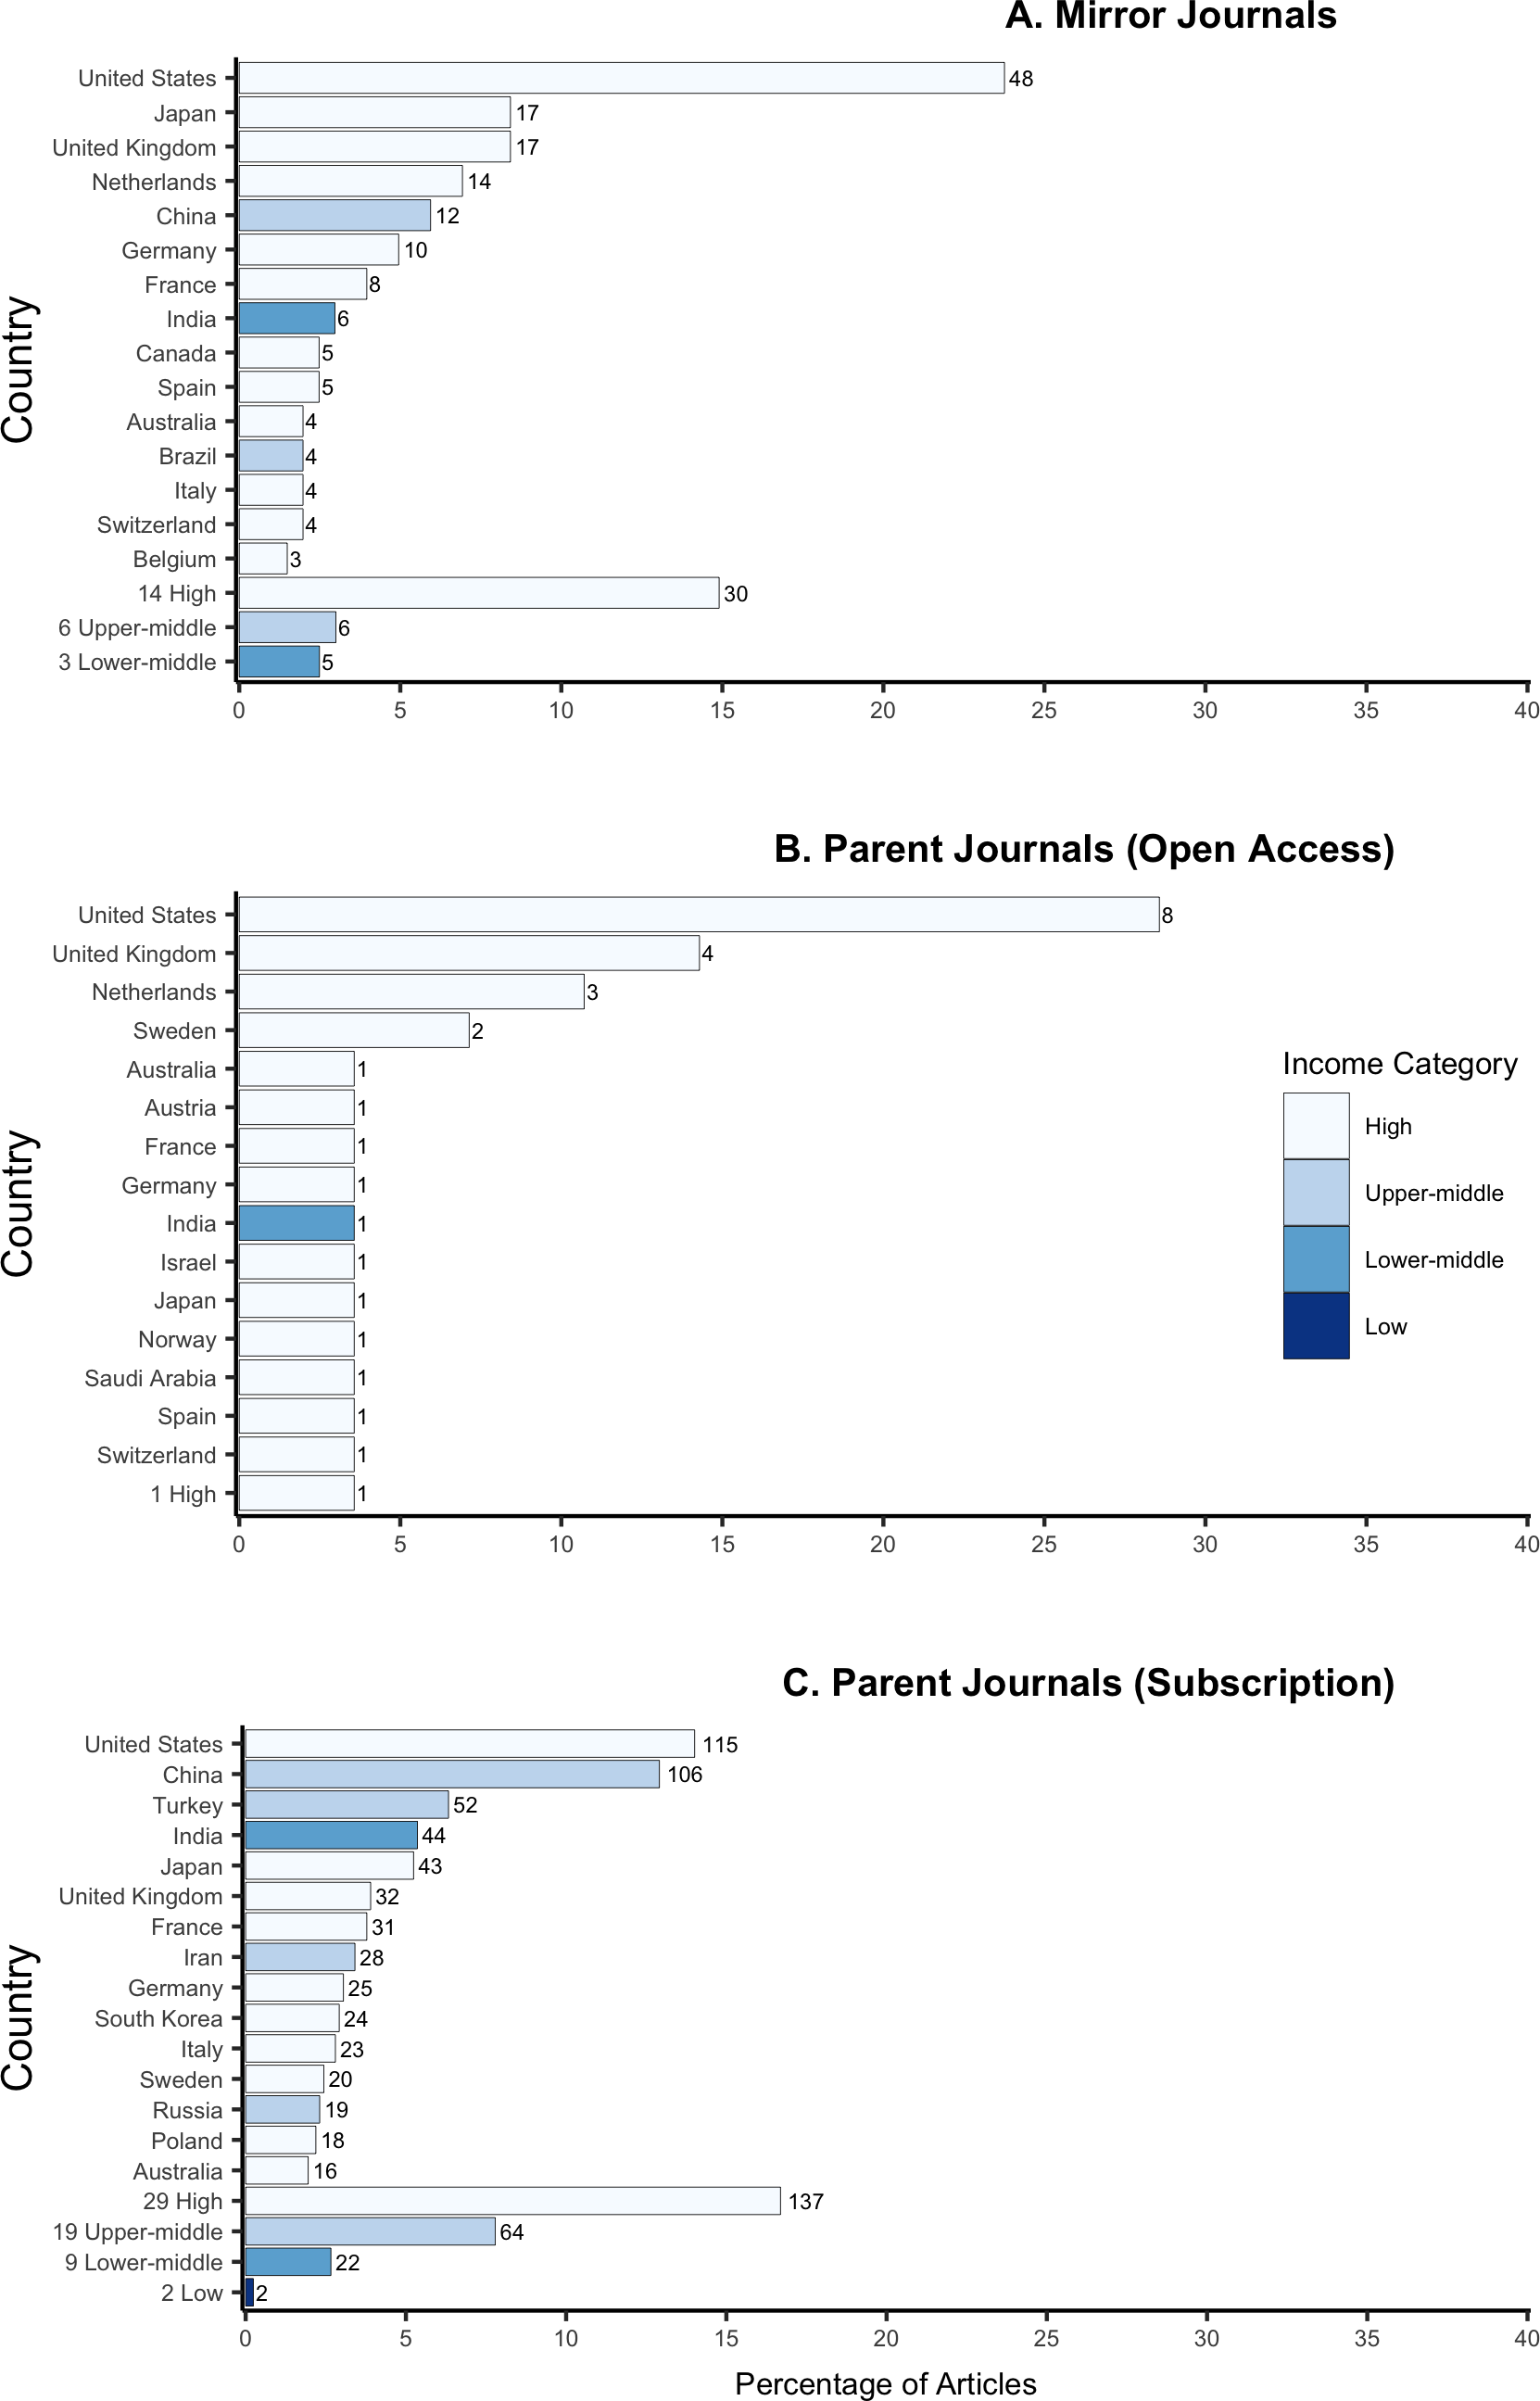
\includegraphics{Smith_etal_APC_ms_files/figure-latex/Fig1-1} 

}

\caption{For single-author papers: (A) the percentage of authors of articles in open access (OA) Mirror journals that are based in different countries, (B) the percentage of authors of OA articles in Parent journals that are based in different countries, and (C) the percentage of authors of non-OA articles in Parent journals that are based in different countries. Numbers adjacent to bars are the number of articles with lead authors based in that country.}\label{fig:Fig1}
\end{figure}

\begin{verbatim}
## TableGrob (3 x 1) "arrange": 3 grobs
##   z     cells    name           grob
## 1 1 (1-1,1-1) arrange gtable[layout]
## 2 2 (2-2,1-1) arrange gtable[layout]
## 3 3 (3-3,1-1) arrange gtable[layout]
\end{verbatim}

\begin{figure}

{\centering 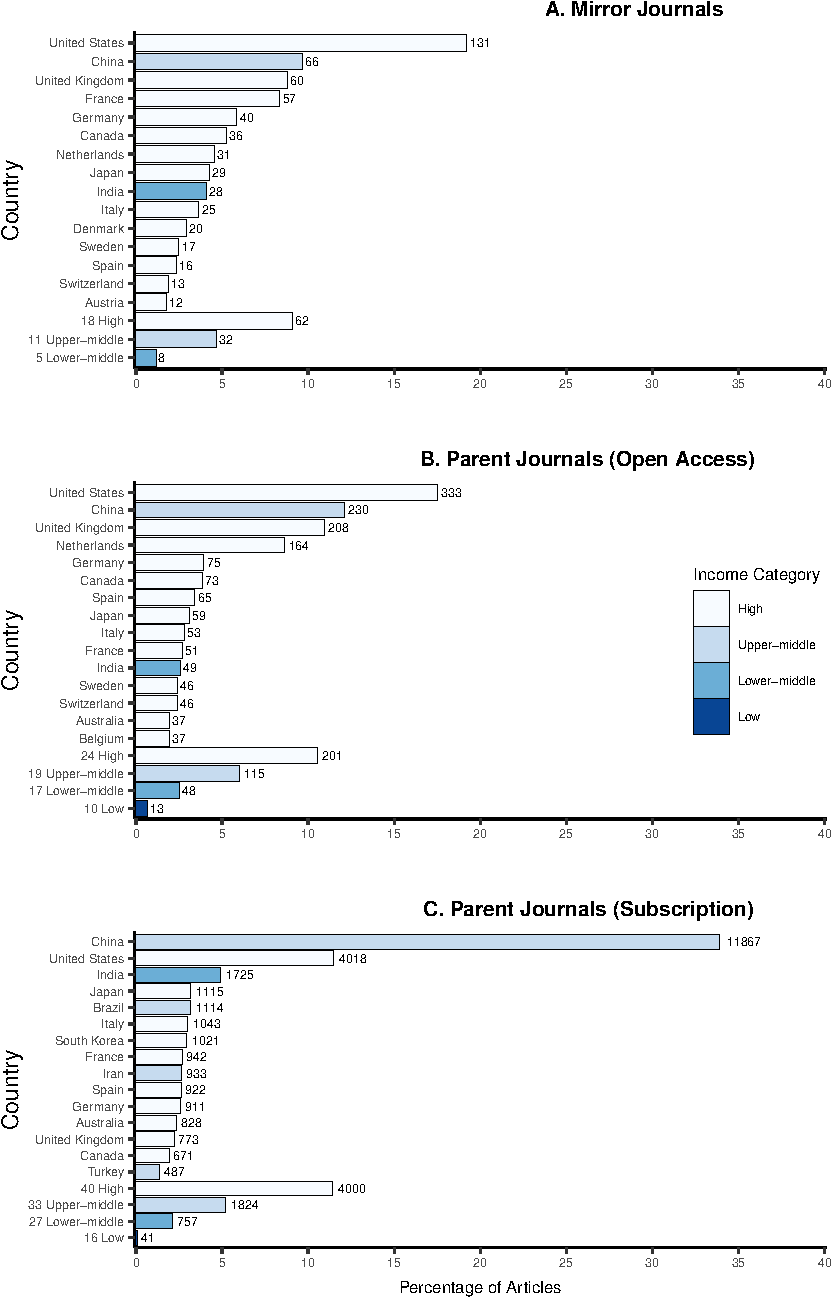
\includegraphics{Smith_etal_APC_ms_files/figure-latex/Fig2-1} 

}

\caption{For coauthored papers: (A) the percentage of authors of articles in open access (OA) Mirror journals that are based in different countries, (B) the percentage of authors of OA articles in Parent journals that are based in different countries, and (C) the percentage of authors of non-OA articles in Parent journals that are based in different countries. Numbers adjacent to bars are the number of articles with lead authors based in that country.}\label{fig:Fig2}
\end{figure}

\begin{verbatim}
## TableGrob (3 x 1) "arrange": 3 grobs
##   z     cells    name           grob
## 1 1 (1-1,1-1) arrange gtable[layout]
## 2 2 (2-2,1-1) arrange gtable[layout]
## 3 3 (3-3,1-1) arrange gtable[layout]
\end{verbatim}

\begin{figure}

{\centering 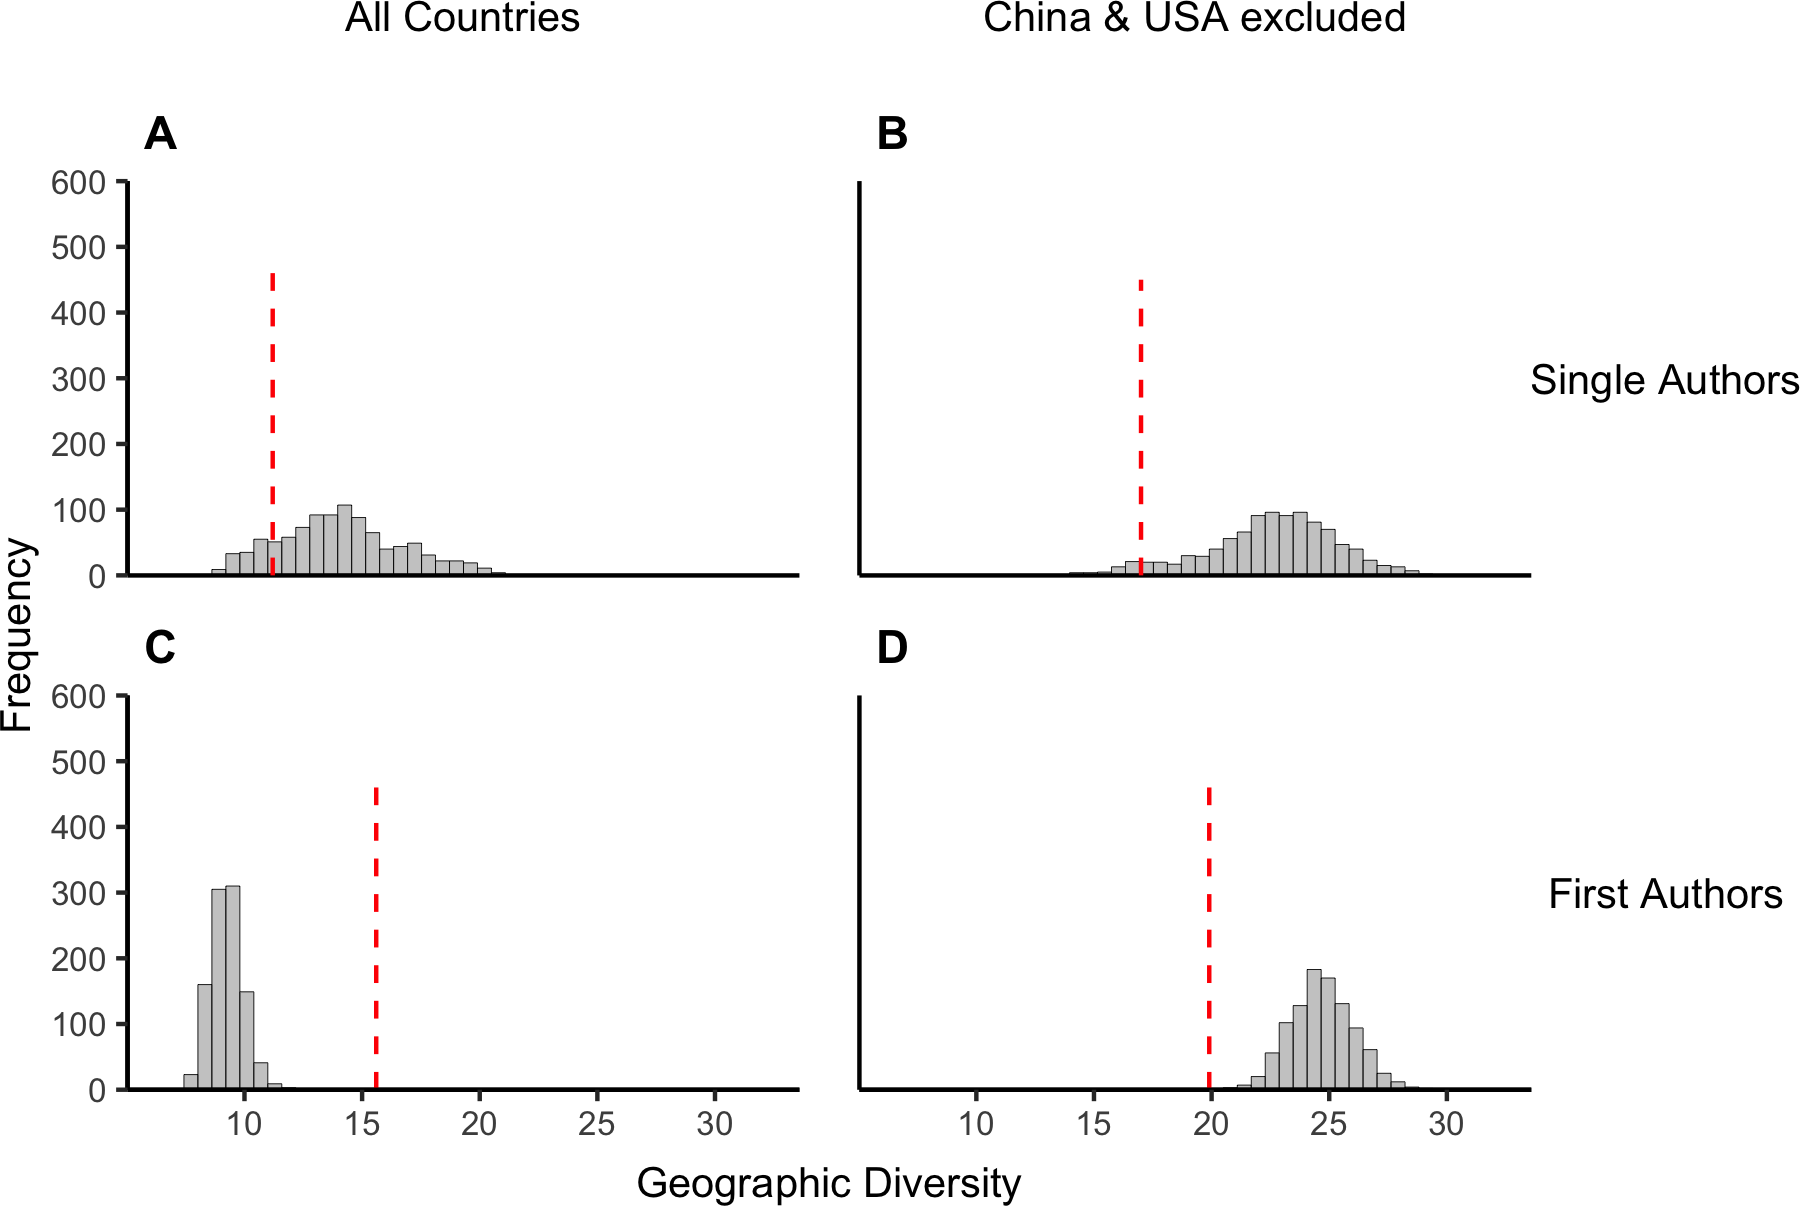
\includegraphics{Smith_etal_APC_ms_files/figure-latex/Fig3-1} 

}

\caption{Geographic Diversity ($D_2$) of authors publishing N =  975  articles in Mirror journals (dashed line) and 1000 collections of N =  975  non-OA articles in Parent journals (sampled from N =  34400  articles by bootstrapping).}\label{fig:Fig3}
\end{figure}

\begin{figure}

{\centering 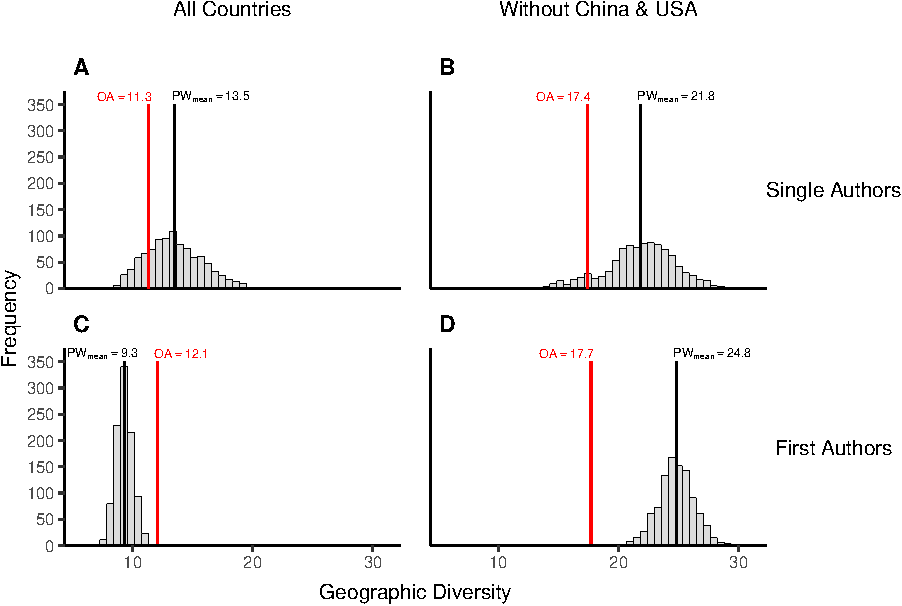
\includegraphics{Smith_etal_APC_ms_files/figure-latex/Fig4-1} 

}

\caption{Percentage of first authors that are based in different global regions. The dashed line is the value for N =  975  articles in open access (OA) Mirror journals; histograms are values for 1000 identically sized collections of non-OA articles from Parent journals (sampled by bootstrapping from N =  34400  articles). All countries, including the USA and China, are included.}\label{fig:Fig4}
\end{figure}

\begin{figure}

{\centering 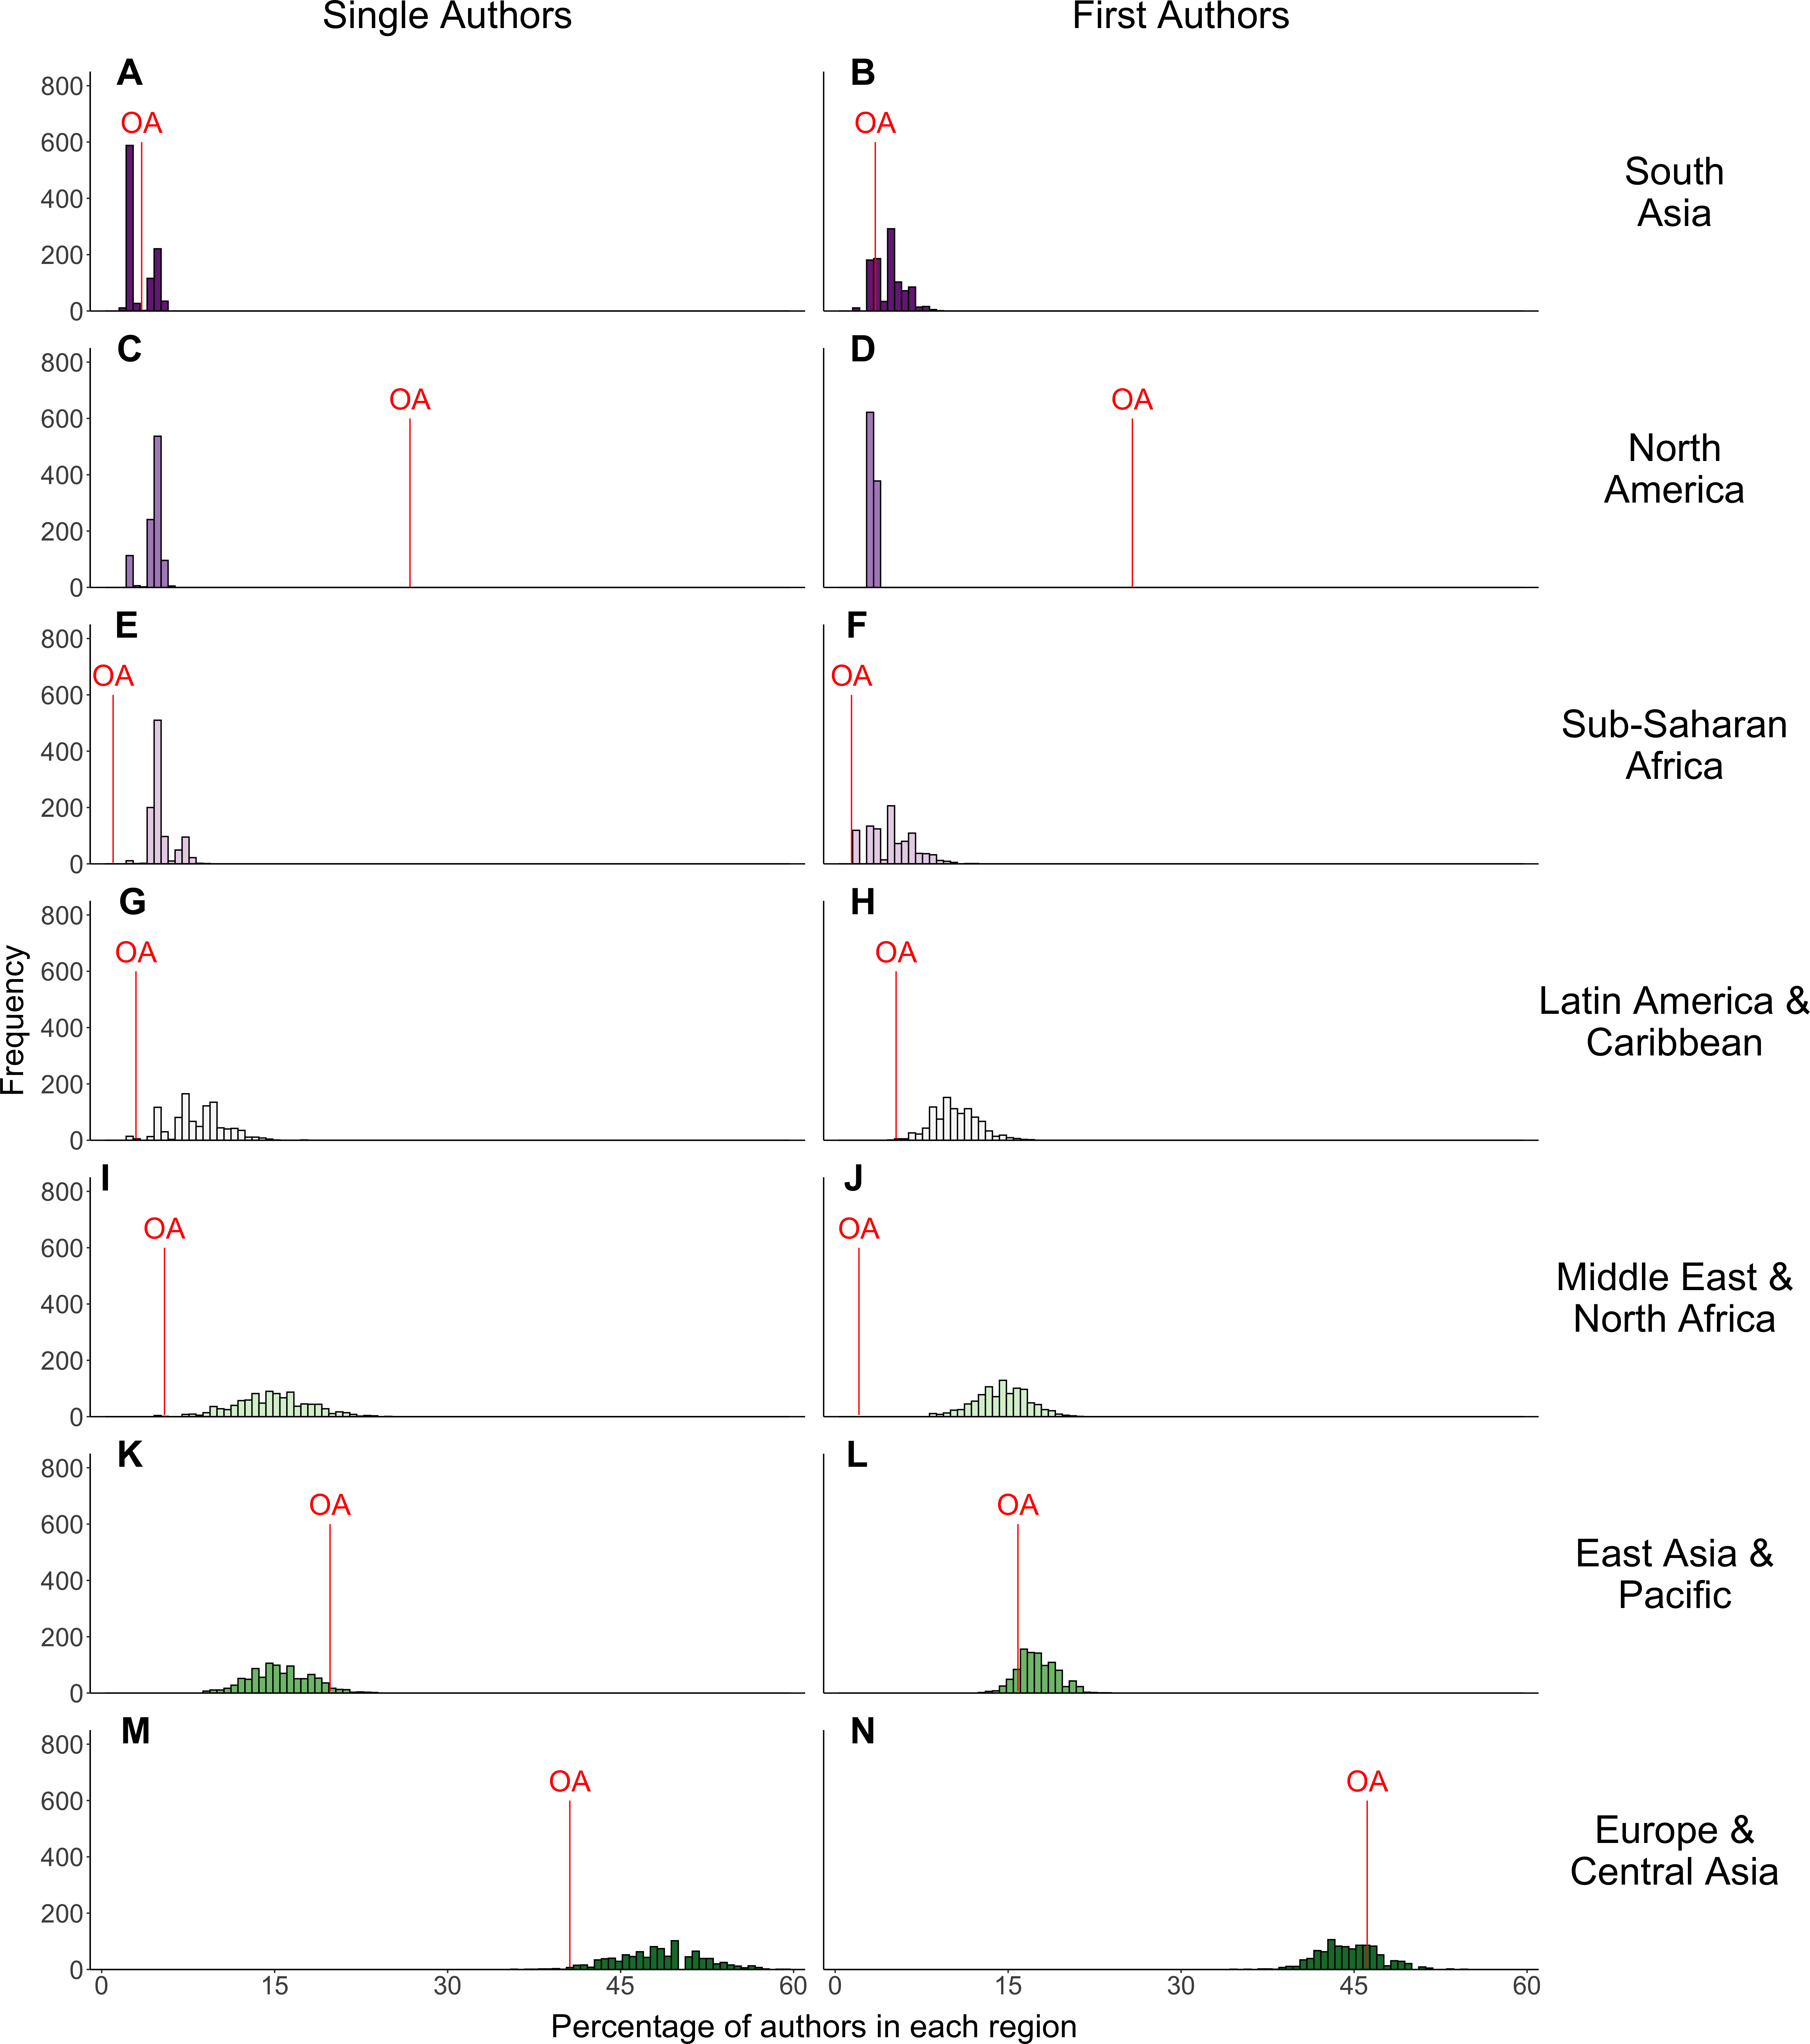
\includegraphics{Smith_etal_APC_ms_files/figure-latex/Fig5-1} 

}

\caption{Percentage of first authors that are based in different World Bank Lending Groups. The dashed line is the value for N =  975  articles in open access (OA) Mirror journals; histograms are values for 1000 identically sized collections of non-OA articles from Parent journals (sampled by bootstrapping from N =  34400  articles). All countries, including the USA and China, are included.}\label{fig:Fig5}
\end{figure}

\begin{figure}

{\centering 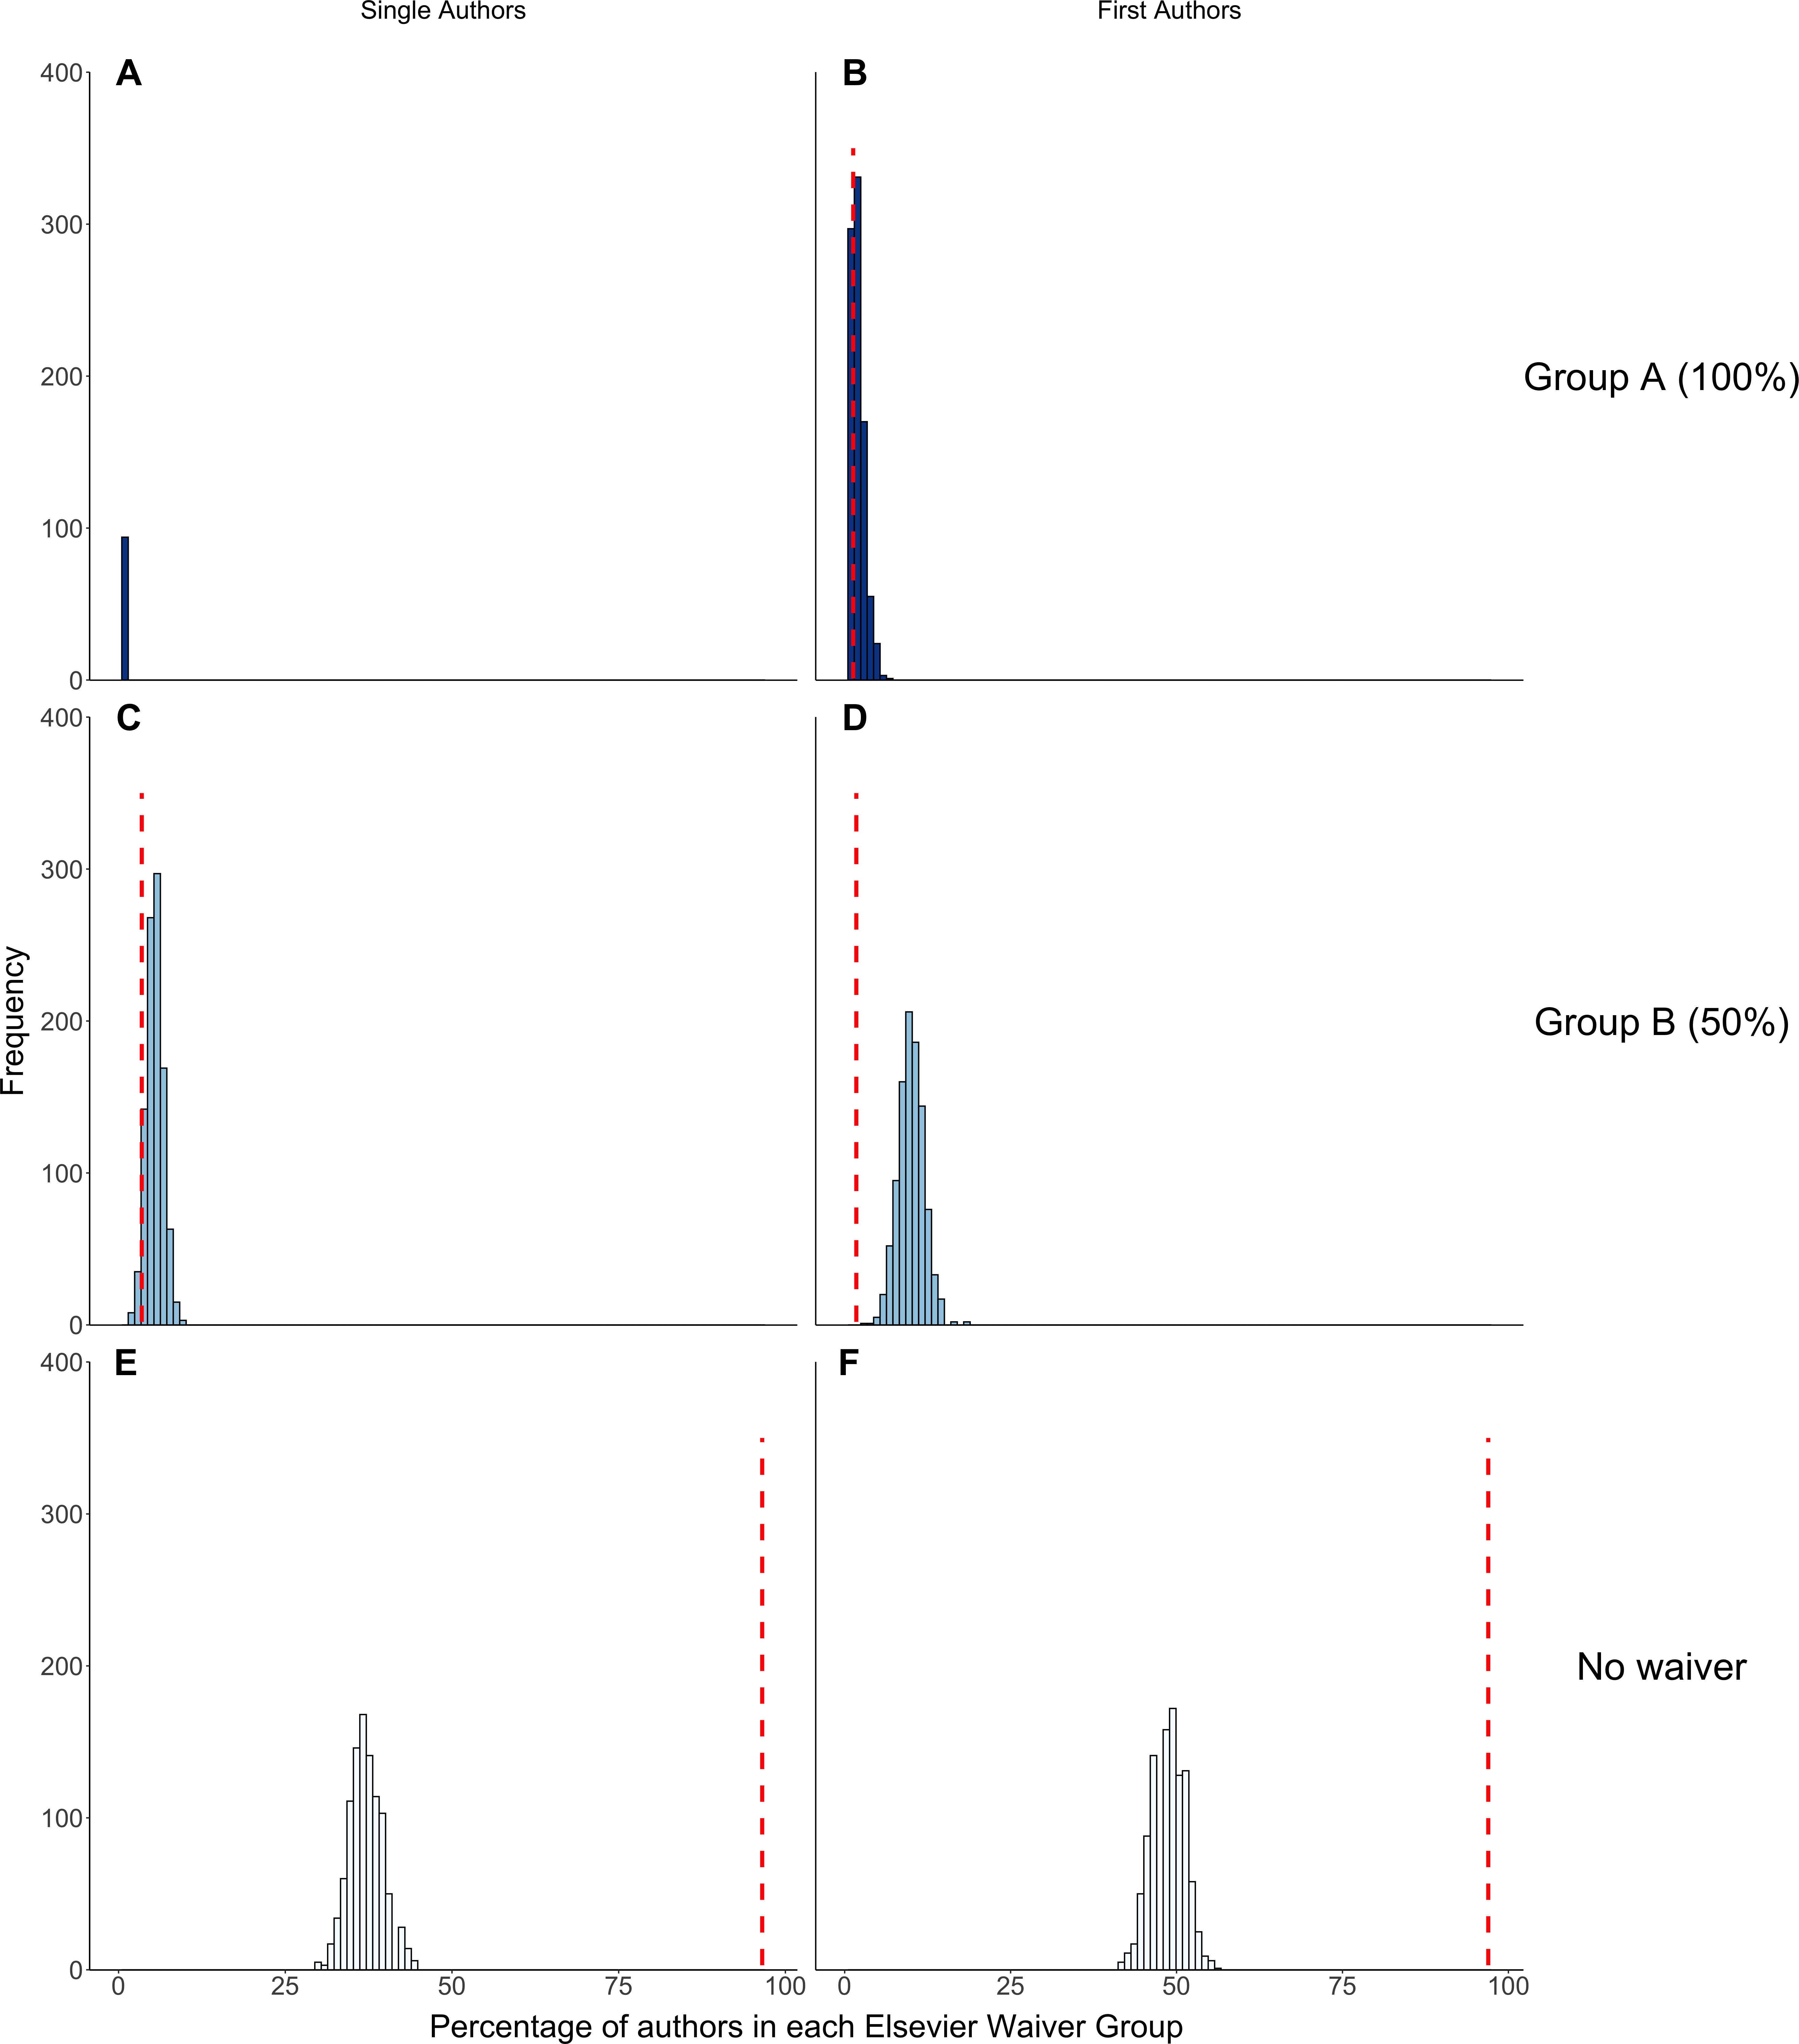
\includegraphics{Smith_etal_APC_ms_files/figure-latex/Fig6-1} 

}

\caption{Percentage of first authors that are based in different Elsevier Waiver Groups. The solid line is the value for N =  975  articles in Mirror journals; histograms are values for 1000 identically sized collections of subscription articles from Parent journals (sampled by bootstrapping from N =  34400  articles).}\label{fig:Fig6}
\end{figure}

\begin{figure}

{\centering 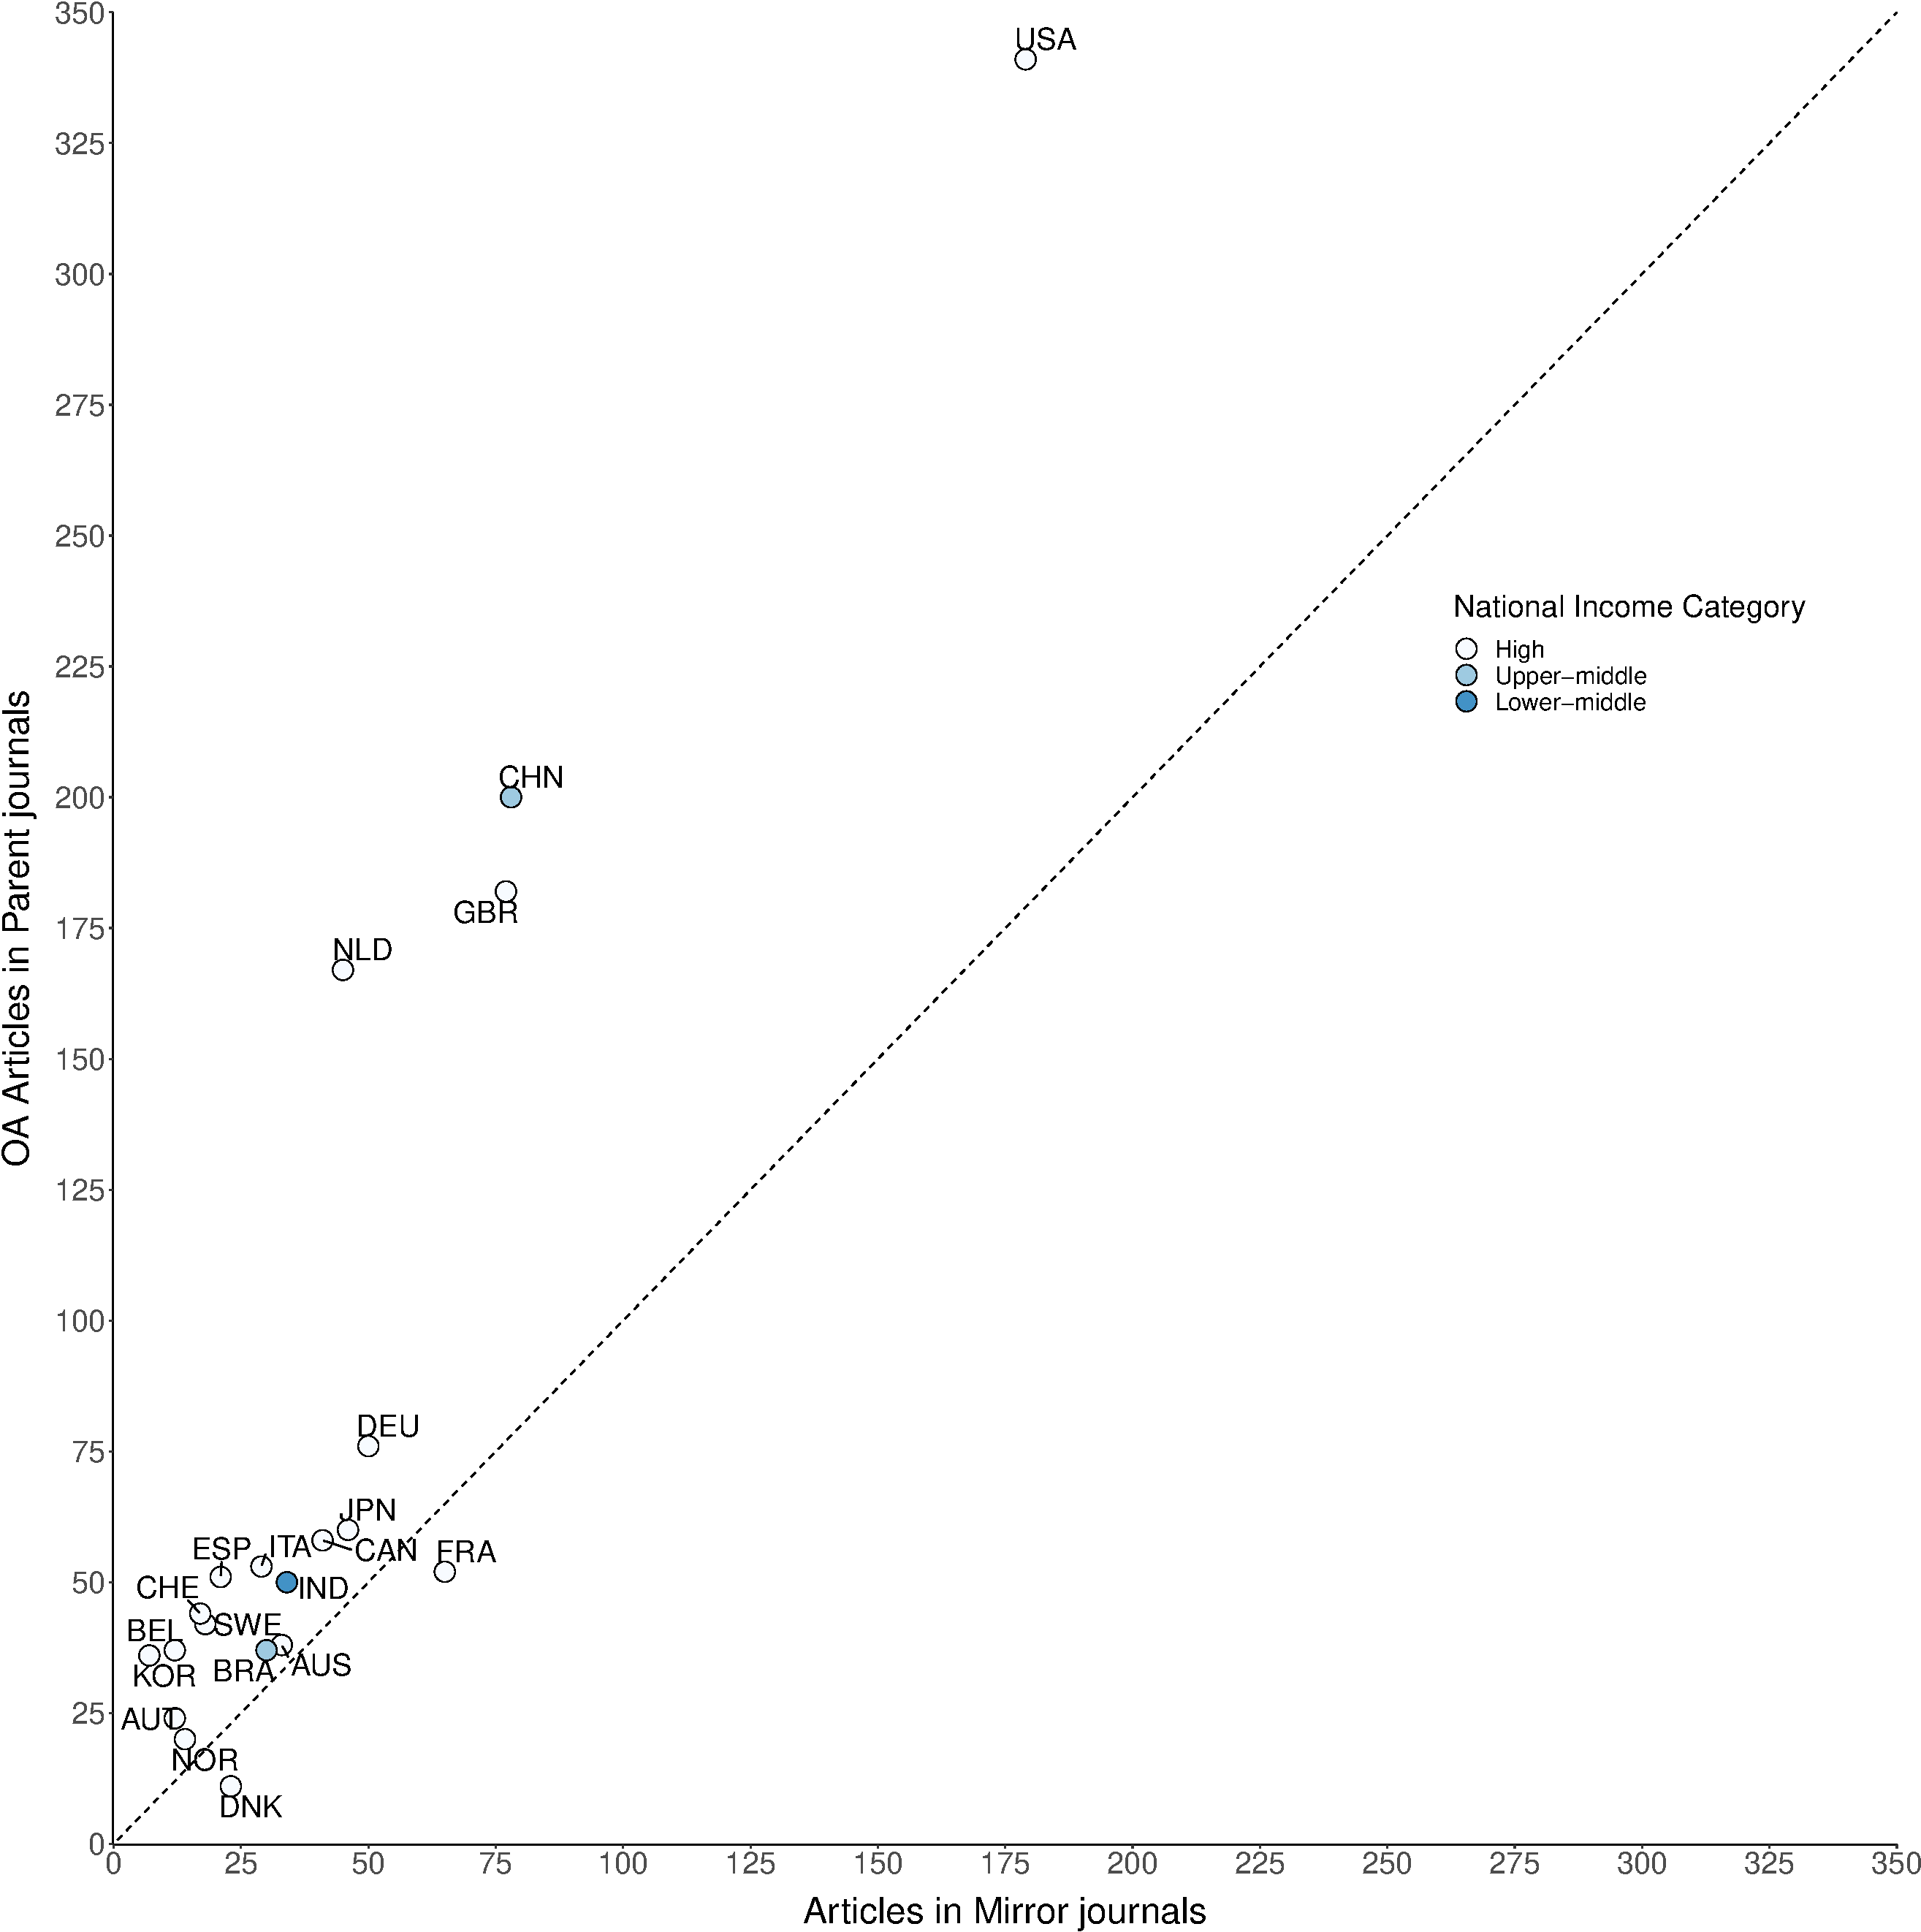
\includegraphics{Smith_etal_APC_ms_files/figure-latex/Fig7-1} 

}

\caption{For the 20 countries publishing the most open access (OA) articles, the number of OA articles published in Mirror Journals vs. OA articles published in Parent journals. Abbreviations: DNK=Denmark, AUT=Austria, NOR=Norway, KOR=South Korea, SWE=Sweden, BEL=Belgium, CHE=Switzerland, ESP=Spain, CAN=Canada, ITA=Italy, DEU=Germany, IND=India, JPN=Japan, BRA=Brazil, AUS=Australia, FRA=France, NLD=Netherlands, GBR=Great Britain, CHN=China, USA=United States of America.)}\label{fig:Fig7}
\end{figure}

\begin{table}

\caption{\label{tab:Table1}Parent journals published by Elsevier included in this study, the number of open access (OA) and non-OA articles they published during our focal time-frame, the number of articles published in each Mirror journal during the same time period, and the article processing charge (APC) charged by each journal for OA publication. With two exceptions the titles of Parent and Mirror journals are identical except for the 'X' at the end of Mirror versions (e.g., Research Policy X, Optical Materials X).}
\resizebox{\linewidth}{!}{
\fontsize{12}{14}\selectfont
\begin{tabular}[t]{lccccc}
\toprule
\multicolumn{1}{c}{ } & \multicolumn{2}{c}{Parent Journal} & \multicolumn{1}{c}{Mirror Journal} & \multicolumn{2}{c}{APC (US\$)} \\
\cmidrule(l{3pt}r{3pt}){2-3} \cmidrule(l{3pt}r{3pt}){4-4} \cmidrule(l{3pt}r{3pt}){5-6}
Title & Subscription & Open Access & Open Access & Mirror & Parent\\
\midrule
Analytica Chimica Acta & 1289 & 8 & 19 & 1850 & 3500\\
Atherosclerosis & 265 & 127 & 5 & 2308 & 3200\\
Atmospheric Environment & 1015 & 41 & 67 & 1400 & 1400\\
Biochimie$^{1}$ & 835 & 71 & 49 & 1318 & 2880\\
Biosensors \& Bioelectronics & 1170 & 0 & 9 & 3500 & 4080\\
Chaos, Solitons \& Fractals & 673 & 0 & 15 & 2200 & 2200\\
Chemical Engineering Science & 1022 & 22 & 45 & 3500 & 3500\\
Chemical Physics Letters & 1137 & 15 & 23 & 3050 & 3050\\
Contraception & 183 & 16 & 21 & 3200 & 3200\\
Cytokine & 425 & 47 & 7 & 3400 & 3400\\
Ecological Engineering & 437 & 18 & 13 & 2600 & 3400\\
Energy Conversion \& Management & 1713 & 29 & 17 & 3100 & 3100\\
European J of Obstetrics, Gyn, \& Repro Bio & 527 & 36 & 84 & 2500 & 2500\\
Expert Systems With Applications & 1084 & 22 & 10 & 2200 & 2640\\
Food Chemistry & 3028 & 49 & 44 & 2800 & 2800\\
Gene & 1079 & 14 & 21 & 3400 & 3400\\
International J of Pharmaceutics & 1293 & 36 & 38 & 3700 & 3700\\
J of Asian Earth Sciences & 602 & 6 & 10 & 2600 & 2600\\
J of Biomedical Informatics & 108 & 132 & 15 & 2350 & 2800\\
J of Biotechnology & 301 & 16 & 10 & 2820 & 3200\\
J of Computational Physics & 970 & 25 & 35 & 2800 & 2800\\
J of Dentistry & 208 & 16 & 5 & 3000 & 3000\\
J of Hydrology & 1417 & 42 & 37 & 3200 & 3200\\
J of Non-Crystalline Solids & 750 & 11 & 33 & 2200 & 2200\\
J of Structural Biology & 152 & 37 & 17 & 2750 & 3310\\
Materials Letters & 2494 & 12 & 30 & 2000 & 3100\\
Microelectronic Engineering$^{2}$ & 547 & 26 & 39 & 2020 & 2200\\
Nutrition & 416 & 26 & 2 & 2050 & 2850\\
Optical Materials & 1020 & 32 & 34 & 1500 & 2200\\
Research Policy & 197 & 58 & 2 & 2400 & 2760\\
Respiratory Medicine & 267 & 31 & 14 & 3500 & 3500\\
Sleep Medicine & 401 & 20 & 8 & 3360 & 3900\\
Toxicon & 271 & 7 & 26 & 3300 & 3300\\
Vaccine & 1016 & 482 & 42 & 2450 & 2950\\
Veterinary Parasitology & 221 & 17 & 21 & 3200 & 3000\\
Water Research & 2083 & 187 & 41 & 3750 & 3750\\
World Neurosurgery & 3441 & 29 & 43 & 2600 & 2240\\
Resources, Conservation, \& Recycling & 552 & 69 & 24 & 3500 & 3500\\
\midrule
Total No. of Articles & 34609 & 1832 & 975 &  & \\
\bottomrule
\multicolumn{6}{l}{\rule{0pt}{1em}\textsuperscript{1} OA Mirror title: Biochimie Open}\\
\multicolumn{6}{l}{\rule{0pt}{1em}\textsuperscript{2} OA Mirror title: Micro and Nano Engineering}\\
\end{tabular}}
\end{table}

\begin{table}

\caption{\label{tab:Table2}Geographic Diversity of lead authors publishing Open Access (i.e., OA) articles in Mirror and Parent journals vs. subscription-only, non-OA, articles in Parent journals (Psub). The value for Psub is the mean of 1000 bootstrap-generated article collections identical in size and structure to each OA group with which they are being compared (i.e., OA in Mirror, OA in Parent). Single: authors of single-authored articles; First: first authors of co-authored articles. Note that because  Diversity values are sample-size dependent, it is not appropriate to compare values generated for one comparison with those generated for another (e.g., Single author OA articles in Parent Journals with First author OA articles in Mirror journals).}
\centering
\resizebox{\linewidth}{!}{
\fontsize{12}{14}\selectfont
\begin{tabular}[t]{llrccrcc}
\toprule
\multicolumn{2}{c}{ } & \multicolumn{3}{c}{All Countries} & \multicolumn{3}{c}{China \& USA Excluded} \\
\cmidrule(l{3pt}r{3pt}){3-5} \cmidrule(l{3pt}r{3pt}){6-8}
Author & OA Source & OA & Psub (mean ± SD) & $\hat{P}$ & OA & Psub (mean ± SD) & $\hat{P}$\\
\midrule
Single & Mirror & 11.2 & 14.07 ± 2.58 & 0.15 & 17.0 & 22.55 ± 2.8 & 0.0\\
 & Parent & 7.5 & 9.87 ± 3.21 & 0.23 & 10.0 & 9.85 ± 3.48 & 0.2\\
 &  &  &  &  &  &  & \\
First & Mirror & 15.6 & 9.25 ± 0.69 & 1.00 & 19.9 & 24.69 ± 1.37 & 0.0\\
 & Parent & 13.3 & 11.63 ± 0.55 & 1.00 & 16.4 & 24.35 ± 0.86 & 0.0\\
\bottomrule
\end{tabular}}
\end{table}

\begin{table}

\caption{\label{tab:Table3}Monthly stipends for graduate students in select countries. The value of the stipend in US currency is based on the exchange rate in December 2020.}
\centering
\fontsize{12}{14}\selectfont
\begin{tabular}[t]{lllc}
\toprule
Country & Agency & Degree & Stipend (US\$)\\
\midrule
Brazil & CNPq$^{1}$ & MS/MA & 294\\
 &  & PhD & 431\\
Mexico & CONACYT$^{2}$ & MS/MA & 588\\
 &  & PhD & 783\\
India & SERB$^{3}$ & PhD$^{6}$ & 747\\
 &  & PhD$^{7}$ & 978\\
Indonesia & RISTEKDIKTI$^{4}$ & MS/MA & 195\\
South Africa & NRF$^{5}$ & MS/MA & 670\\
 &  & PhD & 687\\
\bottomrule
\multicolumn{4}{l}{\rule{0pt}{1em}\textsuperscript{1} http://cnpq.br/apresentacao13/}\\
\multicolumn{4}{l}{\rule{0pt}{1em}\textsuperscript{2} https://www.conacyt.gob.mx/index.php/becas-y-posgrados/becas-nacionales}\\
\multicolumn{4}{l}{\rule{0pt}{1em}\textsuperscript{3} http://www.serb.gov.in/pmfdr.php}\\
\multicolumn{4}{l}{\rule{0pt}{1em}\textsuperscript{4} https://scholarshiproar.com/knb-scholarship/}\\
\multicolumn{4}{l}{\rule{0pt}{1em}\textsuperscript{5} https://www.nrf.ac.za}\\
\multicolumn{4}{l}{\rule{0pt}{1em}\textsuperscript{6} Min. value, Prime Minister’s Doctoral Fellowship}\\
\multicolumn{4}{l}{\rule{0pt}{1em}\textsuperscript{7} Max. value, Prime Minister’s Doctoral Fellowship}\\
\end{tabular}
\end{table}

\begin{table}

\caption{\label{tab:Table4}Percentage of articles in open access (OA) Mirror journals whose authors are based in different World Bank Regions. The value for non-OA articles in Parent journals is the mean percentage of 1000 bootstrap-generated samples identical in size and structure to the articles published in Mirror journals. Single: authors of single-authored papers; First: first authors of co-authored papers.}
\centering
\fontsize{12}{14}\selectfont
\begin{tabular}[t]{lllccc}
\toprule
Countries & Author & Region & non-OA Parent & Mirror & \$\textbackslash{}widehat\{P\}\$\\
\midrule
All Countries & Single & South Asia & 2.98 & 3.48 & 0.72\\
 &  & North America & 4.55 & 26.96 & 1.00\\
 &  & Sub-Saharan Africa & 4.86 & 0.87 & 0.00\\
 &  & Latin America \& Caribbean & 8.73 & 2.61 & 0.01\\
 &  & Middle East \& North Africa & 14.16 & 5.65 & 0.01\\
 &  & East Asia \& Pacific & 15.68 & 18.26 & 0.86\\
 &  & Europe \& Central Asia & 49.06 & 42.17 & 0.02\\
 &  &  &  &  & \\
 & First & South Asia & 4.73 & 3.27 & 0.12\\
 &  & North America & 3.30 & 22.43 & 1.00\\
 &  & Sub-Saharan Africa & 4.63 & 1.32 & 0.00\\
 &  & Latin America \& Caribbean & 10.45 & 3.70 & 0.00\\
 &  & Middle East \& North Africa & 14.62 & 2.38 & 0.00\\
 &  & East Asia \& Pacific & 17.53 & 20.02 & 0.95\\
 &  & Europe \& Central Asia & 44.76 & 46.88 & 0.79\\
\bottomrule
\end{tabular}
\end{table}

\begin{table}

\caption{\label{tab:Table5}Percentage of articles in open access (OA) mirror journal whose authors are based in countries from different World Bank Lending Groups. The value for non-OA articles in Parent journals is the mean percentage of 1000 bootstrap-generated samples identical in size and structure to the articles published in Mirror journals. Single: authors of single-authored papers; First: first authors of co-authored papers.}
\centering
\fontsize{12}{14}\selectfont
\begin{tabular}[t]{lllccc}
\toprule
Countries & Author & Lending Group & non-OA Parent & Mirror & $\hat{P}$\\
\midrule
All Countries & Single & Lower-middle & 9.14 & 5.22 & 0\\
 &  & Upper-middle & 31.36 & 9.57 & 0\\
 &  & High & 59.24 & 85.22 & 0\\
 &  &  &  &  & \\
 & First & Low & 2.38 & 0.51 & 0\\
 &  & Lower-middle & 13.88 & 4.91 & 0\\
 &  & Upper-middle & 27.75 & 17.06 & 0\\
 &  & High & 56.92 & 77.53 & 0\\
\bottomrule
\end{tabular}
\end{table}

\hypertarget{refs}{}
\begin{CSLReferences}{1}{0}
\leavevmode\hypertarget{ref-appel_adoption_2019}{}%
Appel, A. L., Albagli, S., Appel, A. L., \& Albagli, S. (2019). The adoption of article processing charges as a business model by {Brazilian} open access journals. \emph{Transinformação}, \emph{31}, e180045. \url{https://doi.org/10.1590/2318-0889201931e180045}

\leavevmode\hypertarget{ref-aria_bibliometrix_2017}{}%
Aria, M., \& Cuccurullo, C. (2017). Bibliometrix: {An} {R}-tool for comprehensive science mapping analysis. \emph{Journal of Informetrics}, \emph{11}(4), 959--975. \url{https://doi.org/10.1016/j.joi.2017.08.007}

\leavevmode\hypertarget{ref-bahlai_open_2019}{}%
Bahlai, C., Bartlett, L., Burgio, K., Fournier, A., Keiser, C., Poisot, T., \& Whitney, K. (2019). Open science isn't always open to all scientists. \emph{American Scientist}, \emph{107}(2), 78--82. \url{https://doi.org/10.1511/2019.107.2.78}

\leavevmode\hypertarget{ref-bjork_how_2014}{}%
Björk, B.-C., \& Solomon, D. (2014). How research funders can finance {APCs} in full {OA} and hybrid journals. \emph{Learned Publishing}, \emph{27}(2), 93--103. https://doi.org/\url{https://doi.org/10.1087/20140203}

\leavevmode\hypertarget{ref-brandt_north-south_1980}{}%
Brandt, W. (1980). \emph{North-{South}: A programme for survival: Report of the {Independent} {Commission} on {International} {Development} {Issues}. {Cabridge}, {MA}: {MIT} {Press}; 1980.} Cambridge: MIT Press. Retrieved from \url{https://mitpress.mit.edu/contributors/independent-commission-international-development-issues}

\leavevmode\hypertarget{ref-calver_quantifying_2018}{}%
Calver, M., Bryant, K., \& Wardell-Johnson, G. (2018). Quantifying the internationality and multidisciplinarity of authors and journals using ecological statistics. \emph{Scientometrics}, \emph{115}(2), 731--748. \url{https://doi.org/10.1007/s11192-018-2692-z}

\leavevmode\hypertarget{ref-ciocca_reality_2017}{}%
Ciocca, D. R., \& Delgado, G. (2017). The reality of scientific research in {Latin} {America}; an insider's perspective. \emph{Cell Stress \& Chaperones}, \emph{22}(6), 847--852. \url{https://doi.org/10.1007/s12192-017-0815-8}

\leavevmode\hypertarget{ref-coalitions_addendum_2021}{}%
cOAlitionS. (2021). Addendum to the {cOAlition} {S} {Guidance} on the {Implementation} of {Plan} {S}. Retrieved from \url{https://www.coalition-s.org/addendum-to-the-coalition-s-guidance-on-the-implementation-of-plan-s/}

\leavevmode\hypertarget{ref-cochrane_are_2018}{}%
Cochrane, A. (2018). Are {Mirror} journals a better path to the open access flip? \emph{The Scholarly Kitchen}. Retrieved from \url{https://scholarlykitchen.sspnet.org/2018/10/29/are-mirror-journals-a-better-path-to-the-open-access-flip/}

\leavevmode\hypertarget{ref-coonin_publishing_2009}{}%
Coonin, B., \& Younce, L. (2009). Publishing in open access journals in the social sciences and humanities: {Who}'s doing it and why. In \emph{Pushing the {Edge}: {Proceedings} of the {Fourteenth} {National} {Conference} of the {Association} of {College} and {Research} {Libraries}} (pp. 85--94). Seattle, WA.

\leavevmode\hypertarget{ref-crow_income_2009}{}%
Crow, R. (2009). \emph{Income {Models} for {Open} {Access}: {An} {Overview} of {Current} {Practice}}. Washington D.C.: Scholarly Publishing \& Academic Resources Coalition. Retrieved from \url{http://www.arl.org/sparc}

\leavevmode\hypertarget{ref-dallmeier-tiessen_highlights_2011}{}%
Dallmeier-Tiessen, S., Darby, R., Goerner, B., Hyppoelae, J., Igo-Kemenes, P., Kahn, D., \ldots{} Stelt, W. van der. (2011). Highlights from the {SOAP} project survey. {What} {Scientists} {Think} about {Open} {Access} {Publishing}. \emph{arXiv:1101.5260 {[}Cs{]}}. Retrieved from \url{http://arxiv.org/abs/1101.5260}

\leavevmode\hypertarget{ref-davis_open_2011}{}%
Davis, P. M. (2011). Open access, readership, citations: A randomized controlled trial of scientific journal publishing. \emph{The FASEB Journal}, \emph{25}(7), 2129--2134. \url{https://doi.org/10.1096/fj.11-183988}

\leavevmode\hypertarget{ref-editage_geographic_2018}{}%
Editage. (2018). \emph{Geographic {Trends} in {Attitudes} to {Open} {Access}: {Findings} from the {Editage} {Global} {Author} {Survey} 2018}. Retrieved from \url{https://cdn.editage.com/insights/editagecom/production/Geographic}

\leavevmode\hypertarget{ref-efron_introduction_1994}{}%
Efron, B., \& Tibshirani, R. J. (1994). \emph{An introduction to the bootstrap}. CRC press.

\leavevmode\hypertarget{ref-ellers_gold_2017}{}%
Ellers, J., Crowther, T. W., \& Harvey, J. A. (2017). Gold open access publishing in mega-journals: Developing countries pay the price of {Western} premium academic output. \emph{Journal of Scholarly Publishing}, \emph{49}(1), 89--102. \url{https://doi.org/10.3138/jsp.49.1.89}

\leavevmode\hypertarget{ref-elsevier_eligibility_2020}{}%
Elsevier. (2020). Eligibility for access to {Research4Life}. \emph{Eligibility for access to Research4Life}. Retrieved from \url{https://www.research4life.org/access/eligibility/}

\leavevmode\hypertarget{ref-espin_persistent_2017}{}%
Espin, J., Palmas, S., Carrasco-Rueda, F., Riemer, K., Allen, P. E., Berkebile, N., \ldots{} Bruna, E. M. (2017). A persistent lack of international representation on editorial boards in environmental biology. \emph{PLoS Biology}, \emph{15}(12), e2002760. \url{https://doi.org/10.1371/journal.pbio.2002760}

\leavevmode\hypertarget{ref-eysenbach_citation_2006}{}%
Eysenbach, G. (2006). Citation advantage of open access articles. \emph{PLoS Biology}, \emph{4}(5).

\leavevmode\hypertarget{ref-ezema_open_2017}{}%
Ezema, I. J., \& Onyancha, O. B. (2017). Open access publishing in {Africa}: Advancing research outputs to global visibility. \emph{African Journal of Library, Archives \& Information Science; Ibadan}, \emph{27}(2), 97--115. Retrieved from \url{https://search.proquest.com/docview/2236647453/abstract/70E49C1D2C6144FDPQ/1}

\leavevmode\hypertarget{ref-fonturbel_paywall_2021}{}%
Fontúrbel, F. E., \& Vizentin‐Bugoni, J. (2021). A paywall coming down, another being erected: Open access article processing charges ({APC}) may prevent some researchers from publishing in leading journals. \emph{The Bulletin of the Ecological Society of America}, \emph{102}(1), e01791. https://doi.org/\url{https://doi.org/10.1002/bes2.1791}

\leavevmode\hypertarget{ref-fournier_refsplitr_2020}{}%
Fournier, A. M. v., Boone, M. E., Stevens, F. R., \& Bruna, E. M. (2020). Refsplitr: {Author} name disambiguation, author georeferencing, and mapping of coauthorship networks with {Web} of {Science} data. \emph{Journal of Open Source Software}, \emph{5}(45), 2028. \url{https://doi.org/10.21105/joss.02028}

\leavevmode\hypertarget{ref-fox_patterns_2018}{}%
Fox, C. W., Ritchey, J. P., \& Paine, C. E. T. (2018). Patterns of authorship in ecology and evolution: {First}, last, and corresponding authorship vary with gender and geography. \emph{Ecology and Evolution}, \emph{8}(23), 11492--11507. \url{https://doi.org/10.1002/ece3.4584}

\leavevmode\hypertarget{ref-fox_bootstrapping_2015}{}%
Fox, J. (2015). Bootstrapping regression models. In \emph{Applied regression analysis and generalized linear models.} (3rd ed.). Sage.

\leavevmode\hypertarget{ref-gray_sorry_2020}{}%
Gray, R. J. (2020). Sorry, we're open: {Golden} open-access and inequality in non-human biological sciences. \emph{Scientometrics}, \emph{124}(2), 1663--1675. \url{https://doi.org/10.1007/s11192-020-03540-3}

\leavevmode\hypertarget{ref-harrison_what_2019}{}%
Harrison, P. (2019). What are mirror journals, and can they offer a new world of open access? \emph{Elsevier Connect}. Retrieved from \url{https://www.elsevier.com/connect/what-are-mirror-journals-and-can-they-offer-a-new-world-of-open-access}

\leavevmode\hypertarget{ref-iyandemye_low_2019}{}%
Iyandemye, J., \& Thomas, M. P. (2019). Low income countries have the highest percentages of open access publication: {A} systematic computational analysis of the biomedical literature. \emph{PLOS ONE}, \emph{14}(7), e0220229. \url{https://doi.org/10.1371/journal.pone.0220229}

\leavevmode\hypertarget{ref-jamali_national_2020}{}%
Jamali, H. R., Nicholas, D., Herman, E., Boukacem‐Zeghmouri, C., Abrizah, A., Rodríguez‐Bravo, B., \ldots{} Watkinson, A. (2020). National comparisons of early career researchers' scholarly communication attitudes and behaviours. \emph{Learned Publishing}, \emph{33}(4), 370--384. https://doi.org/\url{https://doi.org/10.1002/leap.1313}

\leavevmode\hypertarget{ref-kozak_publication_2013}{}%
Kozak, M., \& Hartley, J. (2013). Publication fees for open access journals: {Different} disciplines---different methods. \emph{Journal of the American Society for Information Science and Technology}, \emph{64}(12), 2591--2594. \url{https://doi.org/10.1002/asi.22972}

\leavevmode\hypertarget{ref-lawson_fee_2015}{}%
Lawson, S. (2015). Fee {Waivers} for {Open} {Access} {Journals}. \emph{Publications}, \emph{3}(3), 155--167. \url{https://doi.org/10.3390/publications3030155}

\leavevmode\hypertarget{ref-macleavy_unintended_2020}{}%
MacLeavy, J., Harris, R., \& Johnston, R. (2020). The unintended consequences of {Open} {Access} publishing -- {And} possible futures. \emph{Geoforum}, \emph{112}, 9--12. https://doi.org/\url{https://doi.org/10.1016/j.geoforum.2019.12.010}

\leavevmode\hypertarget{ref-magurran_measuring_2004}{}%
Magurran, A. E. (2004). \emph{Measuring biological diversity}. Malden, MA: Blackwell Science Ltd.

\leavevmode\hypertarget{ref-matheka_open_2014}{}%
Matheka, D. M., Nderitu, J., Mutonga, D., Otiti, M. I., Siegel, K., \& Demaio, A. R. (2014). Open access: Academic publishing and its implications for knowledge equity in {Kenya}. \emph{Globalization and Health}, \emph{10}, 26. \url{https://doi.org/10.1186/1744-8603-10-26}

\leavevmode\hypertarget{ref-mckiernan_how_2016}{}%
McKiernan, E. C., Bourne, P. E., Brown, C. T., Buck, S., Kenall, A., Lin, J., \ldots{} Yarkoni, T. (2016). How open science helps researchers succeed. \emph{eLife}, \emph{5}, e16800. \url{https://doi.org/10.7554/eLife.16800}

\leavevmode\hypertarget{ref-morrison_oa_2019}{}%
Morrison, H. (2019). {OA} {Main} 2019: {Dataset}, documentation and open peer review invitation. \emph{Sustaining the Knowledge Commons / Soutenir les savoirs communs}. Retrieved from \url{https://sustainingknowledgecommons.org/2019/11/20/oa-main-2019-dataset-documentation-and-open-peer-review-invitation/}

\leavevmode\hypertarget{ref-ncayiyana_open_2005}{}%
Ncayiyana, D. J. (2005). Open access: Barriers and opportunities for lower-income countries. In \emph{Communication given in the {International} {Seminar} {Open} {Access} for {Developing} {Countries}. {Salvador}: {BIREME}/{PAHO}/{WHO}. {Retrieved} {February}} (Vol. 1, p. 2007).

\leavevmode\hypertarget{ref-nunez_assessing_2019}{}%
Nuñez, M. A., Barlow, J., Cadotte, M., Lucas, K., Newton, E., Pettorelli, N., \& Stephens, P. A. (2019). Assessing the uneven global distribution of readership, submissions and publications in applied ecology: {Obvious} problems without obvious solutions. \emph{Journal of Applied Ecology}, \emph{56}(1), 4--9. \url{https://doi.org/10.1111/1365-2664.13319}

\leavevmode\hypertarget{ref-oksanen_vegan_2019}{}%
Oksanen, J., Blanchet, F. G., Friendly, M., Kindt, R., Legendre, P., McGlinn, D., \ldots{} Wagner, H. (2019). Vegan: {Community} {Ecology} {Package}. {R} package version 2.5-6. Retrieved from \url{https://CRAN.R-project.org/package=vegan}

\leavevmode\hypertarget{ref-openapc_openapc_2020}{}%
OpenAPC. (2020). {OpenAPC}. Retrieved from \url{https://treemaps.intact-project.org/apcdata/openapc/\#journal/period=2018}

\leavevmode\hypertarget{ref-parish_dynamics_2018}{}%
Parish, A. J., Boyack, K. W., \& Ioannidis, J. P. A. (2018). Dynamics of co-authorship and productivity across different fields of scientific research. \emph{PLOS ONE}, \emph{13}(1), e0189742. \url{https://doi.org/10.1371/journal.pone.0189742}

\leavevmode\hypertarget{ref-pavan_article_2018}{}%
Pavan, C., \& Barbosa, M. C. (2018). Article processing charge ({APC}) for publishing open access articles: The {Brazilian} scenario. \emph{Scientometrics}, \emph{117}(2), 805--823. \url{https://doi.org/10.1007/s11192-018-2896-2}

\leavevmode\hypertarget{ref-peterson_open_2013}{}%
Peterson, A., Emmett, A., \& Greenberg, M. (2013). Open {Access} and the {Author}-{Pays} {Problem}: {Assuring} {Access} for {Readers} and {Authors} in the {Global} {Academic} {Community}. \emph{Journal of Librarianship and Scholarly Communication}, \emph{1}(3), eP1064. \url{https://doi.org/10.7710/2162-3309.1064}

\leavevmode\hypertarget{ref-pinfield_medical_2013}{}%
Pinfield, S. (2013). Medical research charities and open access. \emph{Learned Publishing}, \emph{26}(4), 285--302. https://doi.org/\url{https://doi.org/10.1087/20130409}

\leavevmode\hypertarget{ref-piwowar_state_2018}{}%
Piwowar, H., Priem, J., Larivière, V., Alperin, J. P., Matthias, L., Norlander, B., \ldots{} Haustein, S. (2018). The state of {OA}: A large-scale analysis of the prevalence and impact of {Open} {Access} articles. \emph{PeerJ}, \emph{6}, e4375.

\leavevmode\hypertarget{ref-powell_achieving_2020}{}%
Powell, A., Johnson, R., \& Herbert, R. (2020). Achieving an equitable transition to open access for researchers in lower and middle-{Income} countries. \emph{SSRN Electronic Journal}. \url{https://doi.org/10.2139/ssrn.3624782}

\leavevmode\hypertarget{ref-poynder_plan_2019}{}%
Poynder, R. (2019). Plan {S} and the {Global} {South} -- {What} do countries in the {Global} {South} stand to gain from signing up to {Europe}'s open access strategy? \emph{Impact of Social Sciences}. Retrieved from \url{https://blogs.lse.ac.uk/impactofsocialsciences/2019/03/06/plan-s-and-the-global-south-what-do-countries-in-the-global-south-stand-to-gain-from-signing-up-to-europes-open-access-strategy/}

\leavevmode\hypertarget{ref-r_core_team_r_2020}{}%
R Core Team. (2020). \emph{R: {A} {Language} and {Environment} for {Statistical} {Computing}}. Vienna, Austria: R Foundation for Statistical Computing. Retrieved from \url{https://www.R-project.org/}

\leavevmode\hypertarget{ref-rodriguez_awareness_2014}{}%
Rodriguez, J. E. (2014). Awareness and attitudes about open access publishing: A glance at generational differences. \emph{The Journal of Academic Librarianship}, \emph{40}(6), 604--610. \url{https://doi.org/10.1016/j.acalib.2014.07.013}

\leavevmode\hypertarget{ref-rowley_factors_2020}{}%
Rowley, J., Sbaffi, L., Sugden, M., \& Gilbert, A. (2020). Factors influencing researchers' journal selection decisions. \emph{Journal of Information Science}, 0165551520958591. \url{https://doi.org/10.1177/0165551520958591}

\leavevmode\hypertarget{ref-schimanski_evaluation_2018}{}%
Schimanski, L. A., \& Alperin, J. P. (2018). The evaluation of scholarship in academic promotion and tenure processes: {Past}, present, and future. \emph{F1000Research}, \emph{7}, 1605. \url{https://doi.org/10.12688/f1000research.16493.1}

\leavevmode\hypertarget{ref-singh_oa_2019}{}%
Singh, S., \& Morrison, H. (2019). {OA} journals non-charging and charging central trends 2010 -- 2019. \emph{Sustaining the Knowledge Commons / Soutenir les savoirs communs}. Retrieved from \url{https://sustainingknowledgecommons.org/2019/11/23/oa-journals-non-charging-and-charging-central-trends-2010-2019/}

\leavevmode\hypertarget{ref-smith_scientific_2014}{}%
Smith, M. J., Weinberger, C., Bruna, E. M., \& Allesina, S. (2014). The scientific impact of nations: Journal placement and citation performance. \emph{PLoS ONE}, \emph{9}(10). \url{https://doi.org/10.1371/journal.pone.0109195}

\leavevmode\hypertarget{ref-solomon_study_2012}{}%
Solomon, D. J., \& Björk, B.-C. (2012a). A study of open access journals using article processing charges. \emph{Journal of the American Society for Information Science and Technology}, \emph{63}(8), 1485--1495. \url{https://doi.org/10.1002/asi.22673}

\leavevmode\hypertarget{ref-solomon_publication_2012}{}%
Solomon, D. J., \& Björk, B.-C. (2012b). Publication fees in open access publishing: {Sources} of funding and factors influencing choice of journal. \emph{Journal of the American Society for Information Science and Technology}, \emph{63}(1), 98--107. \url{https://doi.org/10.1002/asi.21660}

\leavevmode\hypertarget{ref-stocks_geographical_2008}{}%
Stocks, G., Seales, L., Paniagua, F., Maehr, E., \& Bruna, E. M. (2008). The geographical and institutional distribution of ecological research in the tropics. \emph{Biotropica}, \emph{40}(4), 397--404. \url{https://doi.org/10.1111/j.1744-7429.2007.00393.x}

\leavevmode\hypertarget{ref-tennant_academic_2016}{}%
Tennant, J. P., Waldner, F., Jacques, D. C., Masuzzo, P., Collister, L. B., \& Hartgerink, Chris. H. J. (2016). The academic, economic and societal impacts of {Open} {Access}: An evidence-based review. \emph{F1000Research}, \emph{5}, 632. \url{https://doi.org/10.12688/f1000research.8460.3}

\leavevmode\hypertarget{ref-wang_open_2015}{}%
Wang, X., Liu, C., Mao, W., \& Fang, Z. (2015). The open access advantage considering citation, article usage and social media attention. \emph{Scientometrics}, \emph{103}(2), 555--564. \url{https://doi.org/10.1007/s11192-015-1547-0}

\leavevmode\hypertarget{ref-warlick_factors_2007}{}%
Warlick, S. E., \& Vaughan, K. T. L. (2007). Factors influencing publication choice: Why faculty choose open access. \emph{Biomedical Digital Libraries}, \emph{4}(1), 1--12.

\leavevmode\hypertarget{ref-wickham_welcome_2019}{}%
Wickham, H., Averick, M., Bryan, J., Chang, W., McGowan, L. D., François, R., \ldots{} Yutani, H. (2019). Welcome to the {Tidyverse}. \emph{Journal of Open Source Software}, \emph{4}(43), 1686. \url{https://doi.org/10.21105/joss.01686}

\leavevmode\hypertarget{ref-world_bank_world_2020}{}%
World Bank. (2020). World {Bank} {Country} and {Lending} {Groups}. Retrieved from \url{https://datahelpdesk.worldbank.org/knowledgebase/articles/906519-world-bank-country-and-lending-groups}

\leavevmode\hypertarget{ref-xu_chinese_2020}{}%
Xu, J., He, C., Su, J., Zeng, Y., Wang, Z., Fang, F., \& Tang, W. (2020). Chinese researchers' perceptions and use of open access journals: {Results} of an online questionnaire survey. \emph{Learned Publishing}, \emph{33}(3), 246--258. \url{https://doi.org/10.1002/leap.1291}

\leavevmode\hypertarget{ref-zhou_emergence_2006}{}%
Zhou, P., \& Leydesdorff, L. (2006). The emergence of {China} as a leading nation in science. \emph{Research Policy}, \emph{35}(1), 83--104. \url{https://doi.org/10.1016/j.respol.2005.08.006}

\end{CSLReferences}


\end{document}
